\chapter{Event Reconstruction And Simulation}
\label{EventSelection}
\label{recosim}

An important step in any high energy physics analysis is to reconstruct the hard scatter collision from the small deposits of energy measured in the detector. This chapter describes how each sub-detector is used to reconstruct a physics object, such as an electron or muon, which can be used to classify the event as signal or background. Section~\ref{reconstruction} of this chapter describes how electrons, muons, and calorimeter jets are reconstructed in data and Monte Carlo simulated events. Reconstruction of Monte Carlo events requires simulating the $\dzero$~detector such that each Monte Carlo event reproduces the detector resolution observed in data events. The $\dzero$~detector and trigger simulation is described in Sections~\ref{simulation} and~\ref{triggersim}, respectively. Finally, to correct for inevitable un-modeled effects in the simulation, correction factors must be applied to the Monte Carlo. The measurement of these factors and how they are applied is given in Section~\ref{corrections}.

\section{Object Reconstruction}
\label{objectreco}

The following section describes how physics objects are reconstructed using quantities measured in the detector. Section~\ref{trackreco} describes how charged particle tracks are identified through small energy deposits in the central tracking detectors. Once all tracks have been identified the primary interaction vertex can be reconstructed as described in Section~\ref{pvreco}. Electrons and muons are identified through a series of quality cuts as described in Sections~\ref{electronreco} and~\ref{muonreco}, respectively. Section~\ref{jetreco} explains how jets are identified from showers of electromagnetic and hadronic particles in the calorimeter. Once jets, electrons, and muons have been identified the missing transverse energy can be calculated as the $p_{T}$ imbalance in the event as described in Section~\ref{metreco}. Finally, identification of heavy flavor jets using a neural network is described in Section~\ref{bidreco}.

\label{reconstruction}
\subsection{Tracks}
\label{trackreco}

A track represents the three dimensional path of a charged particle as it traverses the detector. In the presence of a magnetic field, such as the case with the inner $\dzero$~detectors, all electrically charged particles move in a helical trajectory. Five parameters are needed to fully parameterize the helix and it is the task of the track finding algorithms to measure these parameters for all charged particles.

The first step in constructing a track is to form ``hits" where ionizing particles have deposited energy in the tracking detectors. The formation of track hits is described in the $Track~Hit~Clustering$~section below. Once the track hits have been created two algorithms are employed to link them together to create charged particle tracks. The two algorithms are described in the $Histogramming~Track~Finding~Method$ and $Alternative~Algorithm$ sections below. A final set of reconstructed tracks is formed by a global track reconstruction algorithm that combines the tracks found by the two previously mentioned algorithms.

\subsubsection{Track~Hit~Clustering}

Building a track begins with forming hits in both the SMT and CFT tracking detectors. A hit in the SMT detector is characterized by the deposition of energy in a silicon strip left by an ionizing particle. If the resulting collected charge is above threshold (to reduce noise hits), a hit is registered. If an adjacent silicon strip also registers a hit the two hits are combined. This process is repeated for any adjacent strip which registers a hit. The center of the SMT hit is given by the charge weighted average of the central position of each silicon strip\footnote{Because the SMT detector is immersed in a magnetic field the electron-positron pairs created in the silicon will drift at an angle with respect to electric field lines within the silicon. This angle, known as the Lorentz angle, is corrected for when calculating the center of the SMT hit.}. A hit in the CFT is formed when two fibers in each super layer register scintillation light indicating the presence of a charge particle traversing the fibers. Because the fibers have a relative $3^{\circ}$~orientation, the $x-y$~coordinates are calculated as the intersection of two scintillating fibers. 

\subsubsection{Histogramming Track Finding Method (HTF)}
\label{htf}

The histogramming track finding (HTF)~\cite{htf} method is based on the principle that a particle which produces many hits in the transverse plane (x-y) will have a unique curvature and azimuthal angle. This method transforms (x-y) hits in the SMT and CFT and into a new plane defined by the curvature, $\rho$, and azimuthal angle, $\phi$. Hits from the same particle will produce a peak in the $\rho-\phi$~space, whereas random hits will uniformly populate the space. An example of this procedure, known as a Hough transformation, for a 1.5~GeV muon track is shown in Fig.~\ref{histogramming}. A histogram is created of the hits in the new $\rho-\phi$ space and is processed through a two-dimensional Kalman filter, which attempts to remove "noisy" tracks with large track errors as well as incorporate detector geometry and material density. The result of the filter is a set of smoothed tracks whose track parameters have been re-fit with smaller errors. The longitudinal coordinate information is included by creating a new histogram in a space defined by the radial distance to the beam axis and the $z$~coordinate. A second Hough transformation is performed into the $(z_{0},C)$ plane, where $z_{0}$ is the intersection of the track along the beam axis and $C$ is the track inclination defined as $\frac{dr}{dz}$. The newly formed tracks are extrapolated either inward toward the SMT if the track finding began in the CFT or outward toward the CFT if the track finding began in the inner SMT detector.

\begin{figure}[!h!tbp]
\begin{center}
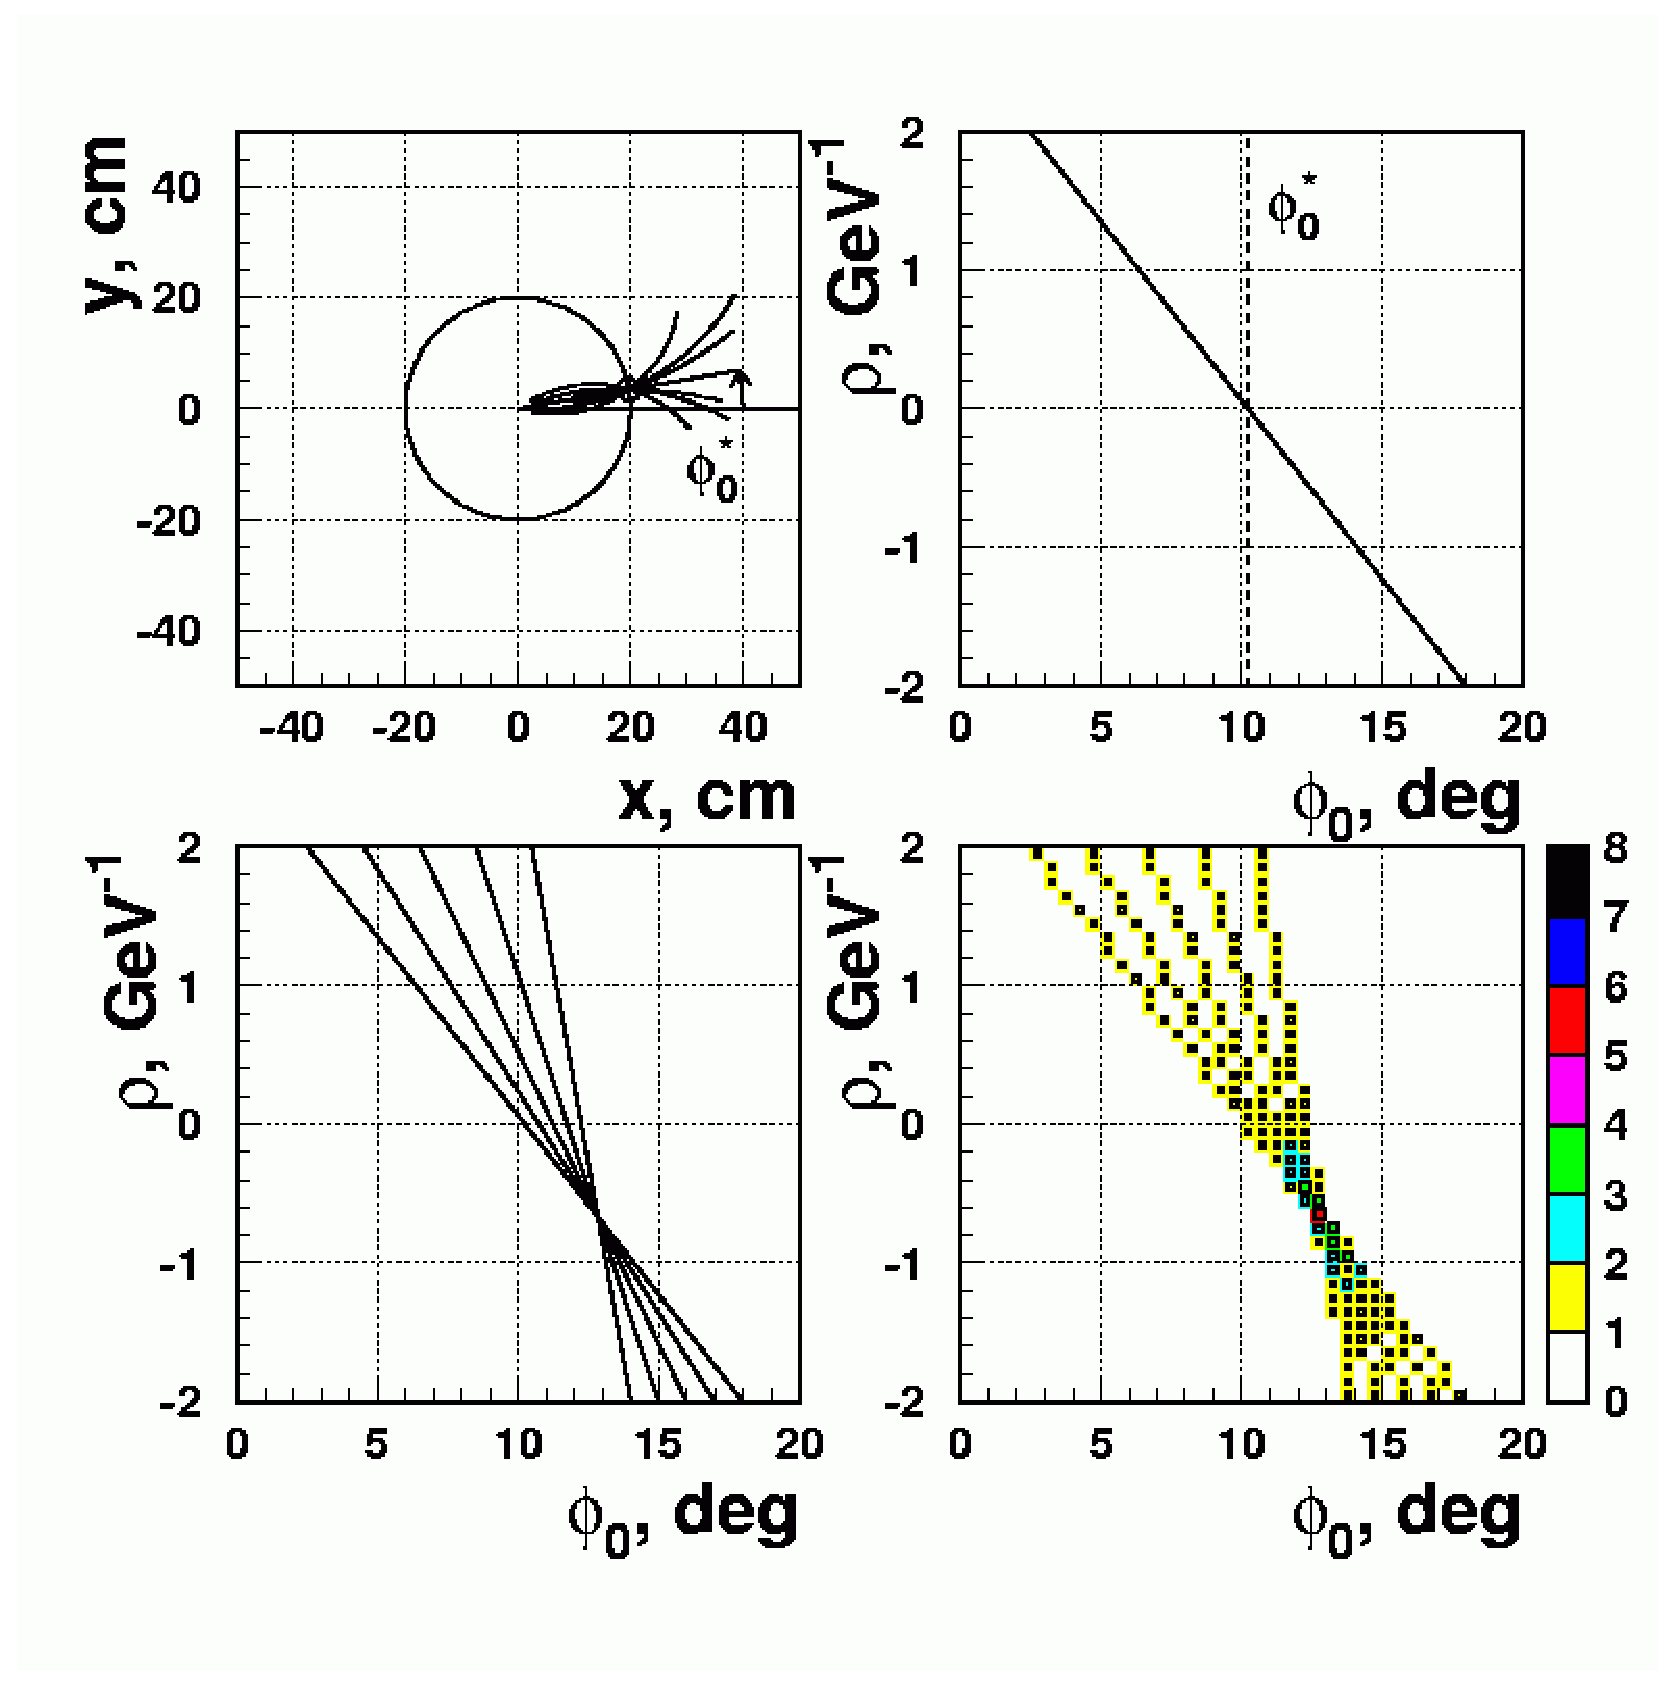
\includegraphics[width=0.75\textwidth]{eps/Reco/htf.eps}
\end{center}
\vspace{-0.1in}
\caption{This histogramming track finding technique shown for an example of a single 1.5 GeV track of 5 hits. (a) The family of trajectories containing a given hit. (b) The geometric place of all trajectories containing a given hit in parameters space. (c) Curves from different hits intersect at one point corresponding to the track parameters. (d) The point of intersection can be seen as a peak in the ($\rho$,~$\phi$) histogram~\cite{htf}.}
\label{histogramming}
\end{figure}


\subsubsection{Alternative Algorithm Tracking (AA)}
\label{aa}

The alternative algorithm (AA)~\cite{aa} track finding method is based on a seed hit in one layer of the detector and building a track by incrementally including more layers of the SMT and CFT detectors. The algorithm takes SMT hits in the innermost layers and adds additional layers if the resulting extrapolated track radius of curvature is greater than $30$~cm, which indicates the track must have $p_{T}>180$~MeV. All possible combinations that meet these requirements are stored. The algorithm also allows for missing hits in the SMT or CFT if a hit in one of the outer layers is consistent with a previously found track. Also allowed are ``CFT-only" tracks built from seeds in the CFT detector that have less than 3 hits in the SMT detector. Allowing tracks to be built in this manner dramatically increases the overall track finding efficiency of the algorithm.


\subsection{Primary Interaction Vertex}
\label{pvreco}

The primary interaction vertex is defined as the three-dimensional location of the hard scatter interaction. The hard scatter interaction vertex is very important to locate to allow discrimination of physics objects resulting from the $\ppbar$~collision and objects created from noise in the detector or other low energy inelastic $\ppbar$~collisions.

Primary interaction vertices are found using the adaptive primary vertex algorithm~\cite{pv}. This algorithm attempts to assign all tracks with $p_{T}>0.5$~GeV and at least two SMT hits to a vertex where the extrapolated track paths intersect. The result of this first pass fit to the primary vertex is a $\chi^{2}$ for each track hypothesis. The algorithm then attempts a second pass fit to the primary vertex except this time each track receives a weight, shown in Eq.~\ref{pvweight}, that includes the $\chi^{2}$ of the previous track fit.

\begin{equation}
\label{pvweight}
w_{i} = \frac{1}{1+e^{(\chi^{2}_{i} - \chi^{2}_{\rm{cutoff}})/2T}}
\end{equation}

\noindent Where the values for $\chi^{2}_{\rm{cutoff}}$ and T are 16 and 4, respectively. The vertex fitting procedure is repeated until the difference of weights from the previous iteration for each track is less than $10^{-4}$.

The adaptive vertexing algorithm produces a list of possible vertices of which one might be the hard scatter vertex. To determine which vertex is the hard scatter vertex all tracks are assigned a probability to not originate from the hard scatter vertex. This probability, shown in Eq~\ref{trackpv}, is based on the $\log_{10}(p_{T})$ (~F$(p_{T})$~)~distribution for tracks associated with a minimum bias\footnote{A minimum bias vertex is a vertex from an inelastic $\ppbar$~collision.} interaction as determined from Monte Carlo simulation.

\begin{equation}
\label{trackpv}
P(p_{T}) = \frac{\int_{\log_{10}(p_{T})}^{\infty} F(p^{'}_{T})dp^{'}_{T}}{\int_{\log_{10}(0.5)}^{\infty} F(p^{'}_{T})dp^{'}_{T}}
\end{equation}

The individual track probabilities are combined for each track associated to each vertex found by the adaptive vertex algorithm to form a minimum bias vertex probability. The vertex which has the lowest minimum bias probability is selected as the hard scatter vertex. The distribution of this probability for minimum bias and hard scatter vertices is shown in Fig.~\ref{minimum bias}.

\begin{figure}[!h!tbp]
\begin{center}
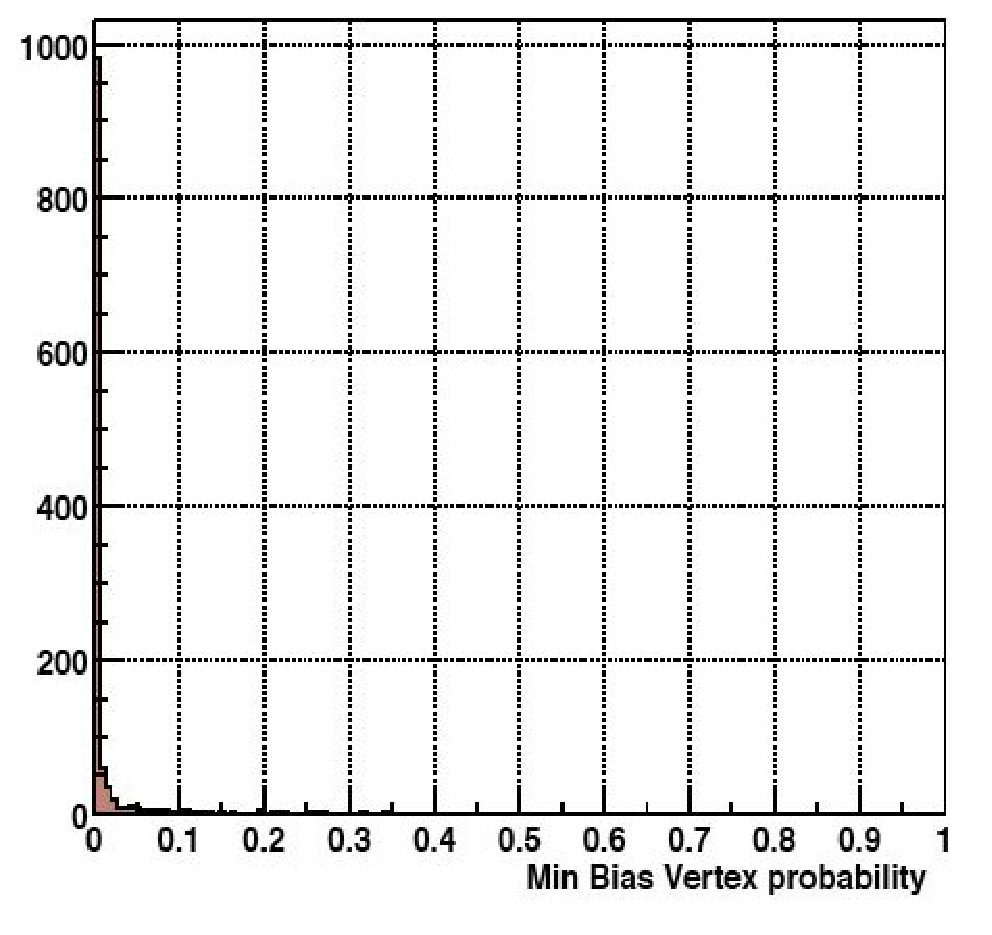
\includegraphics[width=0.49\textwidth]{eps/Reco/MBP_PV.eps}
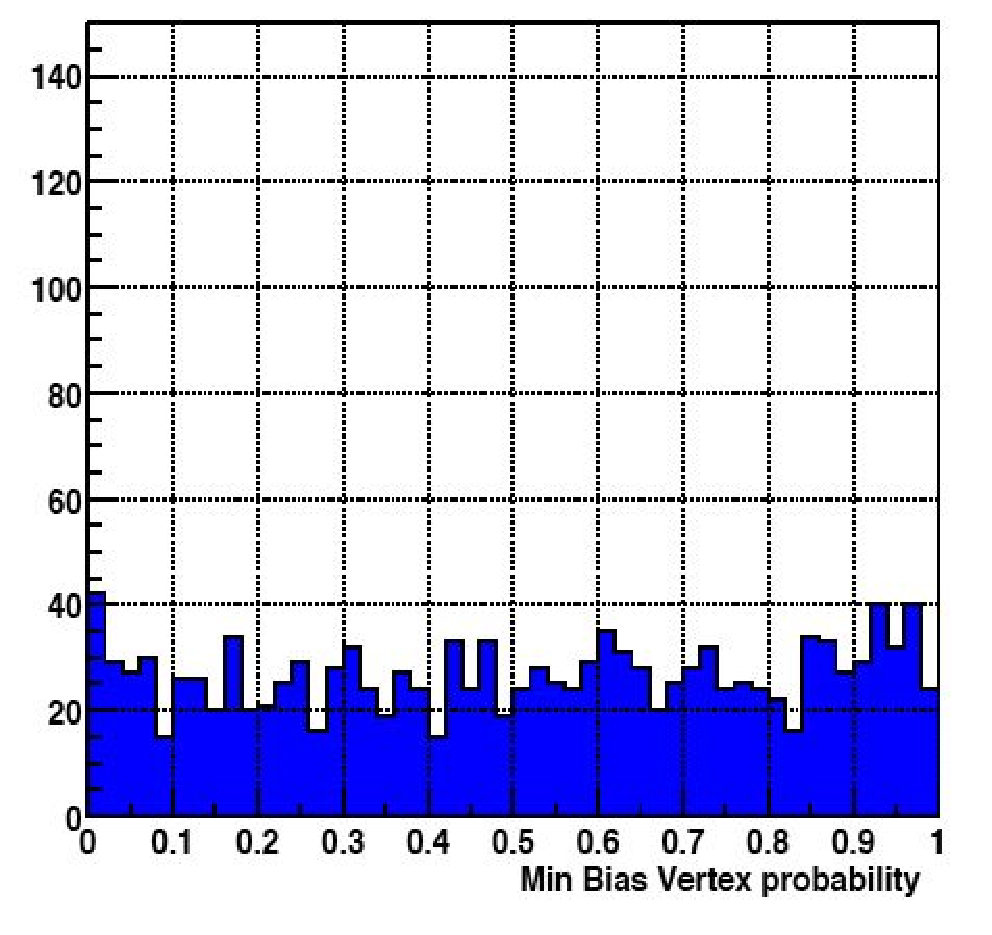
\includegraphics[width=0.49\textwidth]{eps/Reco/MBP_MB.eps}
\end{center}
\vspace{-0.1in}
\caption{Minimum bias probability for the hard scatter vertex (left) and inelastic $\ppbar$ vertices (right). The vertex in the event with the lowest minimum bias probability is selected as the hard scatter vertex~\cite{pv}.}
\label{minimum bias}
\end{figure}


\subsection{Electrons}
\label{electronreco}

Electrons in the $\dzero$~detector are characterized by narrow electromagnetic showers produced in the electromagnetic calorimeter~\cite{electron}. Initial electron candidates are first identified by a cluster of calorimeter towers in the electromagnetic calorimeter. Once a tower is found the electron candidate is defined as the towers surrounding the highest $E_{T}$ tower in a cone of radius 0.4. Since electrons will deposit most of their energy in the inner electromagnetic calorimeter the ratio of the electron candidate energy found in the electromagnetic calorimeter should be greater than $90\%$ of the energy deposited in the electromagnetic calorimeter. The shape of the electromagnetic shower should also be consistent with an electron or photon shower. Electrons are distinct from photons in that they are charged particles thus all electron candidates are required to have a track with $p_{T}>5$~GeV pointing in the direction of the electromagnetic cluster. 
To ensure that the electron is well measured it is also required to be isolated from other electromagnetic clusters. The isolation, shown in Eq.~\ref{fiso}, is defined in terms of the electromagnetic calorimeter towers with $\Delta R<0.2$ and $\Delta R<0.4$ surrounding the electron candidate and is required to be less than 0.15.

\begin{equation}
\label{fiso}
\rm{f_{iso}} = \frac{E_{EM}(\Delta R <  0.4) - E_{EM}(\Delta R <  0.2)}{E_{EM}(\Delta R <  0.4)}
\end{equation}

Finally, to ensure high quality electrons a likelihood discriminant is created using seven variables that will separate electrons from W/Z boson decays (real electrons) from jets with large electromagnetic fractions (fake electrons). Electrons with a likelihood discriminant greater than 0.85 are considered true electrons from a W/Z decay.

\subsection{Muons}
\label{muonreco}

Muon are reconstructed in the $\dzero$~detector by requiring hits in the three layers of the muon system from both the scintillators and wire chambers~\cite{muon}. A muon candidate is required to register at least two wire hits and at least one scintillator hit in the A layer.  At least two wire hits in the B and C layers as well as at least one scintillator hit in this region are also required for the muon. From the hits in the three layers it is possible to construct a local momentum measurement due to the curvature induced by the toroid magnet, however, the resolution of this measurement is quite poor. To improve the resolution, the local muon track is required to be matched with a track found by the global track reconstruction algorithm.

To remove muons produced by cosmic rays the muon candidate is required to be temporally coincident with a bunch crossing. After a bunch crossing is registered the muon candidate is required to hit all three layers within $10$~ns. To further reduce the cosmic ray background the muon track is required to originate from the primary interaction vertex with a relative longitudinal distance less than 1~cm and a transverse distance of closest approach (DCA) less than 0.2 cm if there are no SMT hits and less than 0.02 cm if there is at least one SMT hit.

Finally, an isolation cut is applied to ensure the muon is the product of a $W$ boson decay and not the result of a heavy flavor decay (e.g. $B \rightarrow \mu\nu_{\mu} D$). To remove muons from heavy flavor decays the candidate is required to be isolated ($\Delta R(\mu,\rm{jet}) > 0.5$)~from nearby jets since muons from heavy flavor decays will tend to be found inside or near a jet. To further reject muons from heavy flavor decays, two isolation variables are defined in terms of the muon track $p_{T}$ and the sum of either calorimeter energy or track momentum surrounding the muon momentum vector. The two isolation variables, shown in Eq.~\ref{trackiso} and~\ref{caliso}~are both required to be less than 0.2.

\begin{equation}
\label{trackiso}
f_{\rm{Track~Isolation}}(\mu, \rm{Tracks}) = \frac{1}{p_{T}(\mu)} \times \sum_{\rm{tracks \neq muon~ \Delta R < 0.5 }}p_{T}(\rm{track})
\end{equation}

\begin{equation}
\label{caliso}
f_{\rm{Calorimeter~Isolation}}(\mu, \rm{CalTowers}) = \frac{1}{p_{T}(\mu)} \times \sum_{\rm{cal~tower~0.1 < \Delta R < 0.4 }}E_{T}(\rm{cal~tower})
\end{equation}
%  author = {J. Hays, J. Mitrevski, C. Schwanenberger, T. Toole},


\subsection{Jets}
\label{jetreco}

A jet is defined as a narrow cone of strongly interacting particles produced by the hadronization of strongly interacting particles such as quarks or gluons. A jet will shower in the electromagnetic and hadronic calorimeters and its energy is measured by sampling this shower in the many layers of the $\dzero$~calorimeter. A proper measurement of the jet energy and direction is needed to determine the original quark or gluon energy and momentum.

The Run II improved legacy cone algorithm~\cite{Blazey:2000qt} is used to reconstruct jets in the $\dzero$ calorimeter. This algorithm selects calorimeter towers with transverse energies\footnote{The transverse energy is the energy of the calorimeter tower weighted by the sine of the polar angle $\theta$ of the tower (i.e. $E_{T} = E \times \sin(\theta)$).} greater than $0.5$~GeV as seeds around which the jet is built. The algorithm collects all calorimeter towers in a cone\footnote{The jet cone is defined in terms of rapidity ($y$) and azimuthal angle ($\phi$).} of radius $0.5$ around the seed tower and defines this as the jet candidate if it has $E_{T}>1$~GeV. The central axis of the jet is defined by the $E_{T}$ weighted midpoints of each calorimeter tower. This procedure is repeated throughout the detector until all jets are stable (i.e. the jet axis from one iteration to the next does not change) with a total $E_{T}>6$~GeV. The final step of the jet finding algorithm is to remove overlapping jets. A jet is defined as overlapping if it shares energy with another jet. Two overlapping jets are merged if the overlapping energy is more than half of the individual jet energies. If the overlapping jets are not merged, then they are split into two distinct jets whose total $E_{T}$ and axis are recomputed.

%Cone jets have several advantages both experimentally and theoretically. Since the jets are defined by rapidity and $\phi$, they are invariant under boosts along the longitudinal direction (beam axis). This is important because the longitudinal boost of events at the Tevatron will typically be large with resepect to the $\ppbar$~rest frame. The other advantage of cone jets is they are infrared safe meaning that one can calculate jet properties in the low energy regime of a theory without incurring singularities.

Once the jets have been reconstructed a set of quality criteria are applied to remove fake jets created out of calorimeter noise and remove electromagnetic particles such as electrons and photons. To remove jets created by electromagnetic particles a jet is required to have between 5 and 95$\%$ of its energy deposited in the hadronic calorimeter. Also, a jet is required to be isolated ($\Delta R>0.5$) from all electromagnetic clusters in the detector. To remove fake jets created by calorimeter noise the jet is required to have at least 60$\%$ of its energy deposited in the fine hadronic calorimeter since this detector has higher energy resolution than the coarse hadronic calorimeter. Jets created by a single ``noisy" cell are removed by requiring that more than one calorimeter cell contain at least $90\%$ of the jet energy. Also, to further suppress the effect of a noisy cell the ratio of the most energetic tower to the second most energetic tower must be less than 10.

\subsubsection{Jet Energy Scale Correction}

In reconstructing physics objects in an event, the goal is to measure the four-momenta of the final state particles from the hard scatter collision. For jets this is quite complicated due to the nearly 4 radiation lengths of material that separate the collision center from the calorimeter. It is the goal of the jet energy scale correction to modify the calorimeter jet energies to the parton energy before any interaction with the $\dzero$~detector~\cite{jes}.

The corrected jet energy, which is defined as the energy of a final state parton before interacting with the detector, is given by Eq.~\ref{jes} in terms of five other quantities, which are explained below.

\begin{equation}
\label{jes}
E_{\rm{jet}}^{\rm{corr}} = \frac{E_{\rm{jet}}^{\rm{uncorr}} - \rm{O}}{\rm{F}_{\eta} \times \rm{R} \times \rm{S}}
\end{equation}

\begin{itemize}
\item $E_{\rm{jet}}^{\rm{uncorr}}$ is the uncorrected jet energy as determined by the reconstruction algorithm.

\item O is the offset correction and represents energy that contributes to the jet that is not associated with the hard scatter collision. Two examples of additional sources of energy are electronics noise and additional minimum bias interactions in the same bunch crossing. The offset correction is measured in minimum bias events by summing the energy of calorimeter towers within a jet cone radius. A plot of the offset energy correction as a function of the detector pseudorapidity ($\eta^{\rm{det}}$)\footnote{$\eta^{\rm{det}}$ is the pseudorapidity defined with respect to the detector origin instead of the collision center.} for several primary vertex multiplicities is shown in Fig.~\ref{jesoffset}.

\begin{figure}[!h!tbp]
\begin{center}
\includegraphics[width=0.75\textwidth]{eps/Reco/jes-offset.eps}
\end{center}
\vspace{-0.1in}
\caption{Offset energy correction for jets with a cone radius of 0.5 as a function of $\eta^{det}$~\cite{jes}.}
\label{jesoffset}
\end{figure}

\item F$_{\eta}$ is the relative response of the calorimeter in different $\eta$~regions. This term is designed to cancel the expected non-uniformity of the $\dzero$~calorimeter between the central and endcap  calorimeter cryostats. The relative response is measured using the missing $E_{T}$ projection fraction method in back-to-back one photon with one jet events. In this method the photon is considered perfectly well measured, which implies that that any E$_{T}$ imbalance in the event is an effect of the response. A cartoon of the method is shown in Fig.~\ref{metprojection}.

\begin{figure}[!h!tbp]
\begin{center}
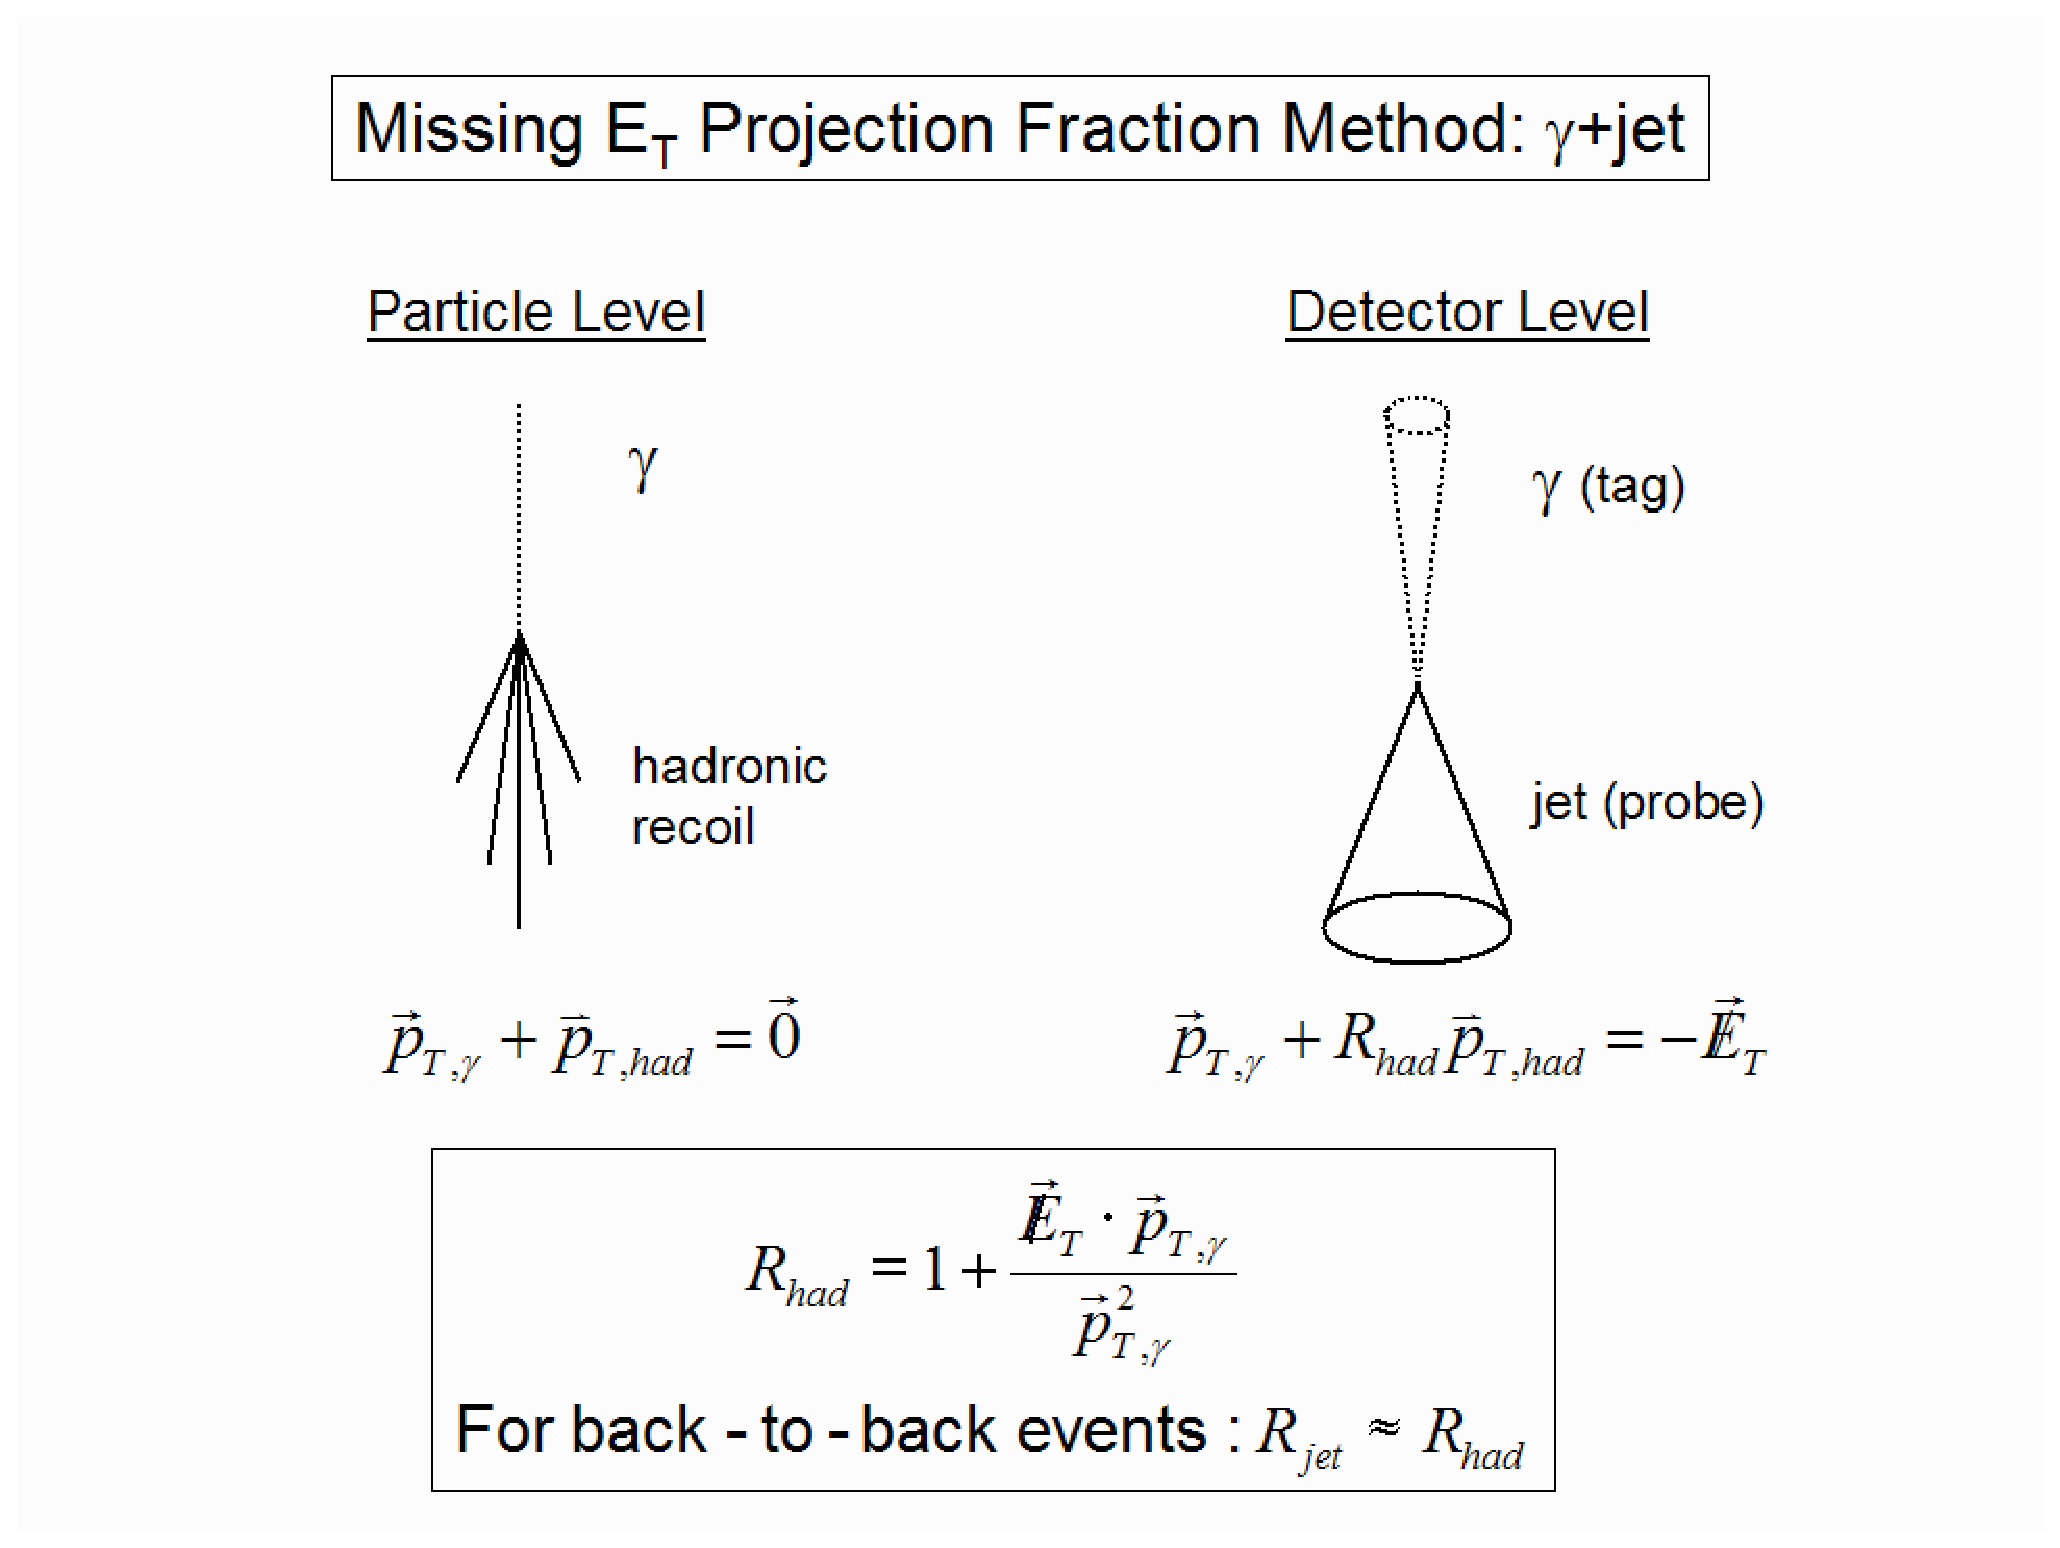
\includegraphics[width=0.75\textwidth]{eps/Reco/JES-relative-method.eps}
\end{center}
\vspace{-0.1in}
\caption{Missing $E_{T}$ ($E_{T}$ imbalance) projection fraction method cartoon~\cite{jes}.}
\label{metprojection}
\end{figure}

By measuring the missing E$_{T}$ and the $p_{T}$ of the photon and jet the response relative to $\eta=0$ can be measured in many regions of $\eta^{\rm{det}}$. The relative response with respect to $\eta=0$~in data is shown in Fig.~\ref{jes-relative}.

\begin{figure}[!h!tbp]
\begin{center}
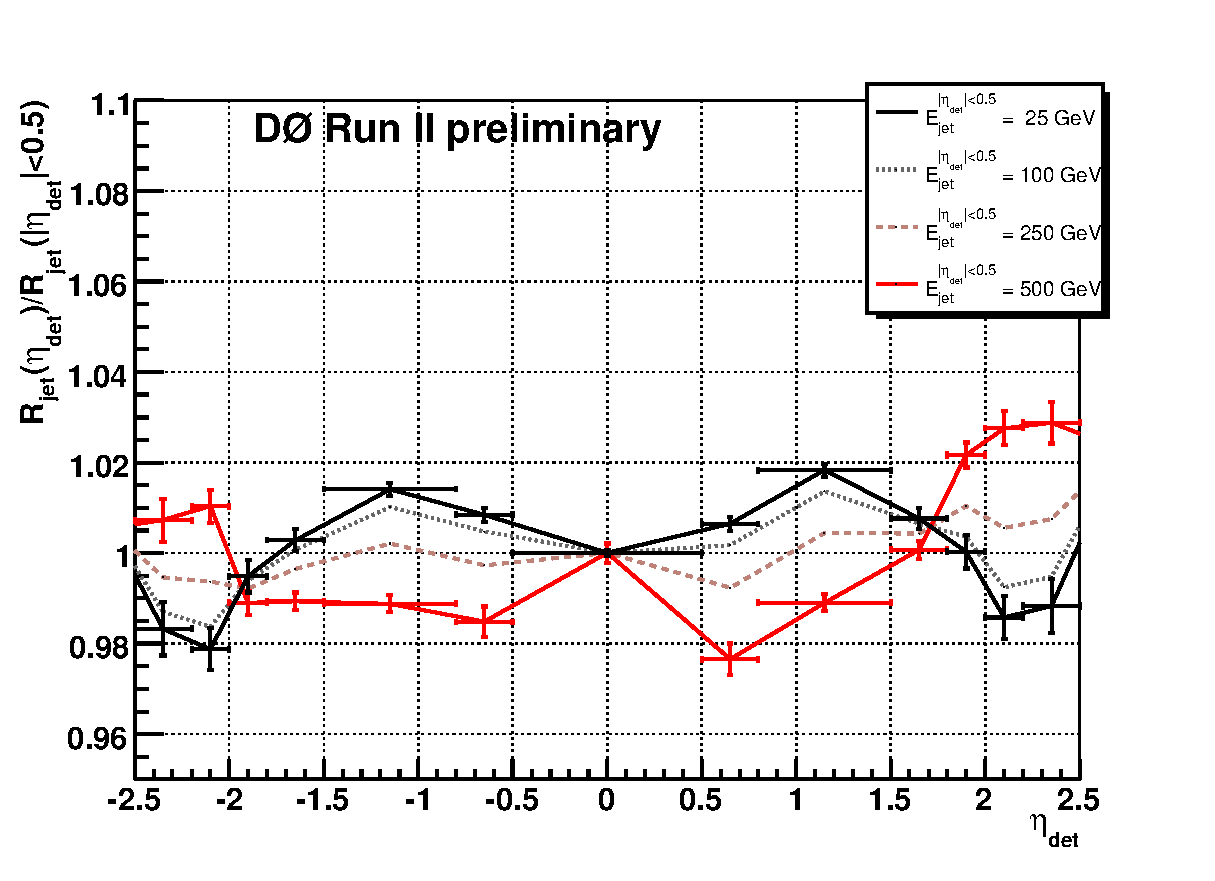
\includegraphics[width=0.75\textwidth]{eps/Reco/JES-relative.eps}
\end{center}
\vspace{-0.1in}
\caption{The relative energy correction for jets with a cone radius of 0.5 as a function of $\eta^{det}$ (right)~\cite{jes}.}
\label{jes-relative}
\end{figure}
 
\item R is the absolute energy response of the calorimeter. This term accounts for energy lost in un-instrumented regions of the detector and the lower energy response of the calorimeter to hadrons compared to electrons or photons. The absolute response is also determined using back-to-back photon+jet events and is measured after the relative response in $\eta$ has been applied. Fig.~\ref{jes-absolute} shows the absolute energy response for different $\eta$ regions to emphasize the uniformity of the calorimeter after applying the relative response term.

\begin{figure}[!h!tbp]
\begin{center}
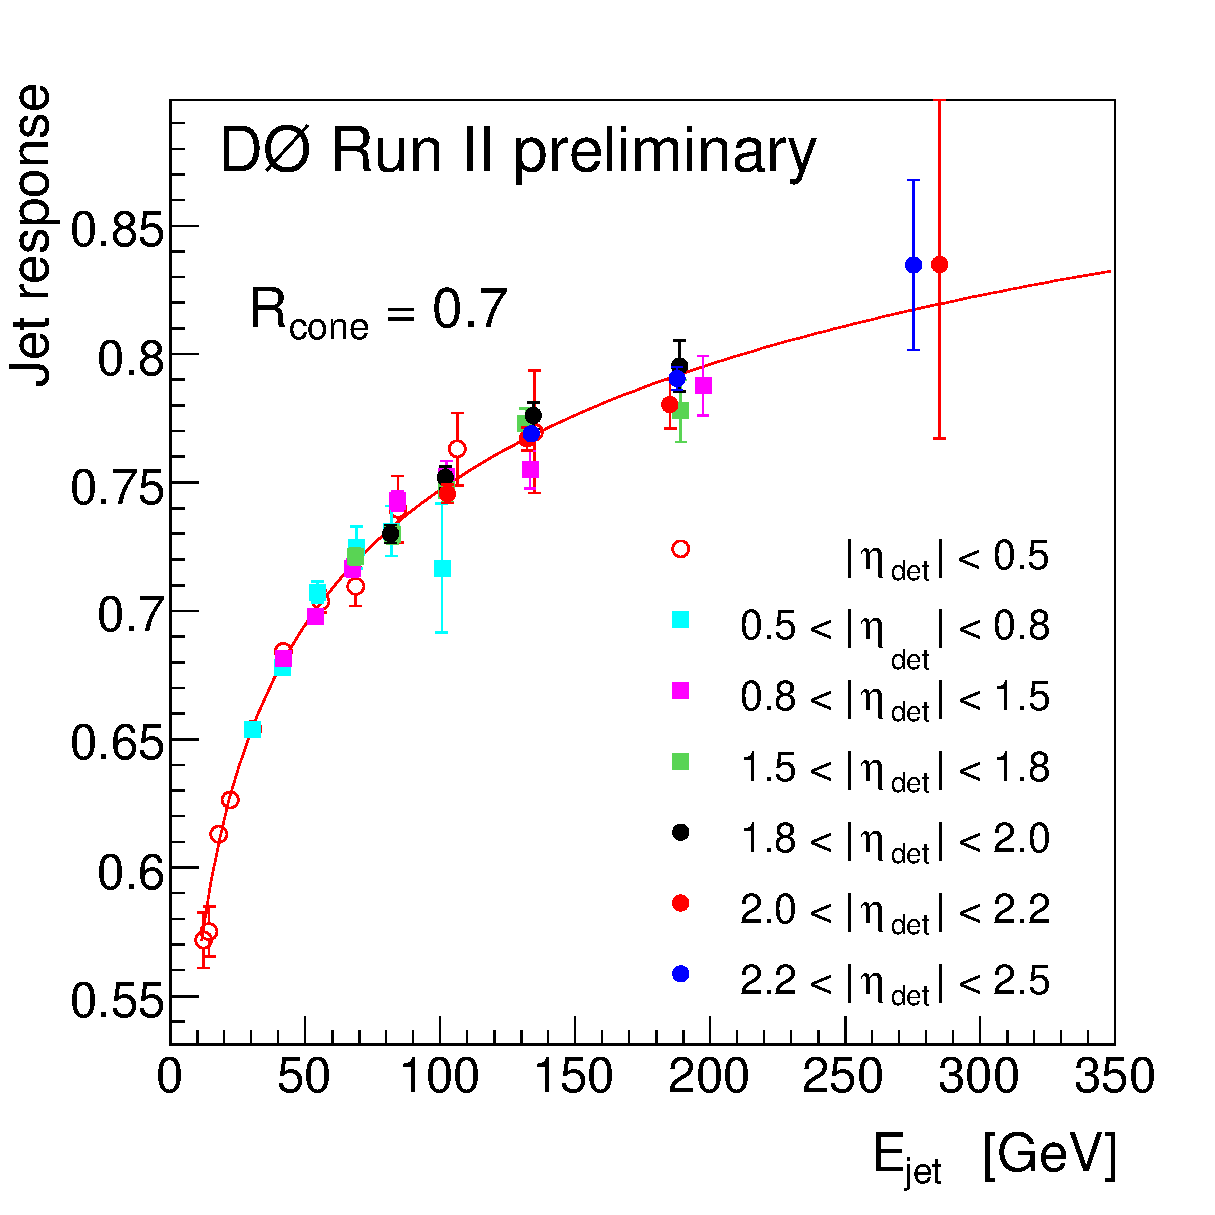
\includegraphics[width=0.75\textwidth]{eps/Reco/JES-absolute.eps}
\end{center}
\vspace{-0.1in}
\caption{Absolute energy response of jets in the calorimeter for several $\eta$ regions~\cite{jes}.}
\label{jes-absolute}
\end{figure}

\item S is the showering correction. This term corrects for energy deposited outside the cone radius of the reconstructed jet or additional energy deposited inside the cone radius as a result of spurious particles in the calorimeter. The showering correction is measured by calculating the total energy deposited inside and outside the jet and taking the ratio of these numbers with the known deposited energy as determined in Monte Carlo events. The calculation in Monte Carlo is done without detector simulation such that the ratio of the two quantities yields the showering correction due to the detector only. Fig.~\ref{jes-shower} shows the showering correction as a function of jet E$_{T}$ for jets in three different $\eta$ regions.

\begin{figure}[!h!tbp]
\begin{center}
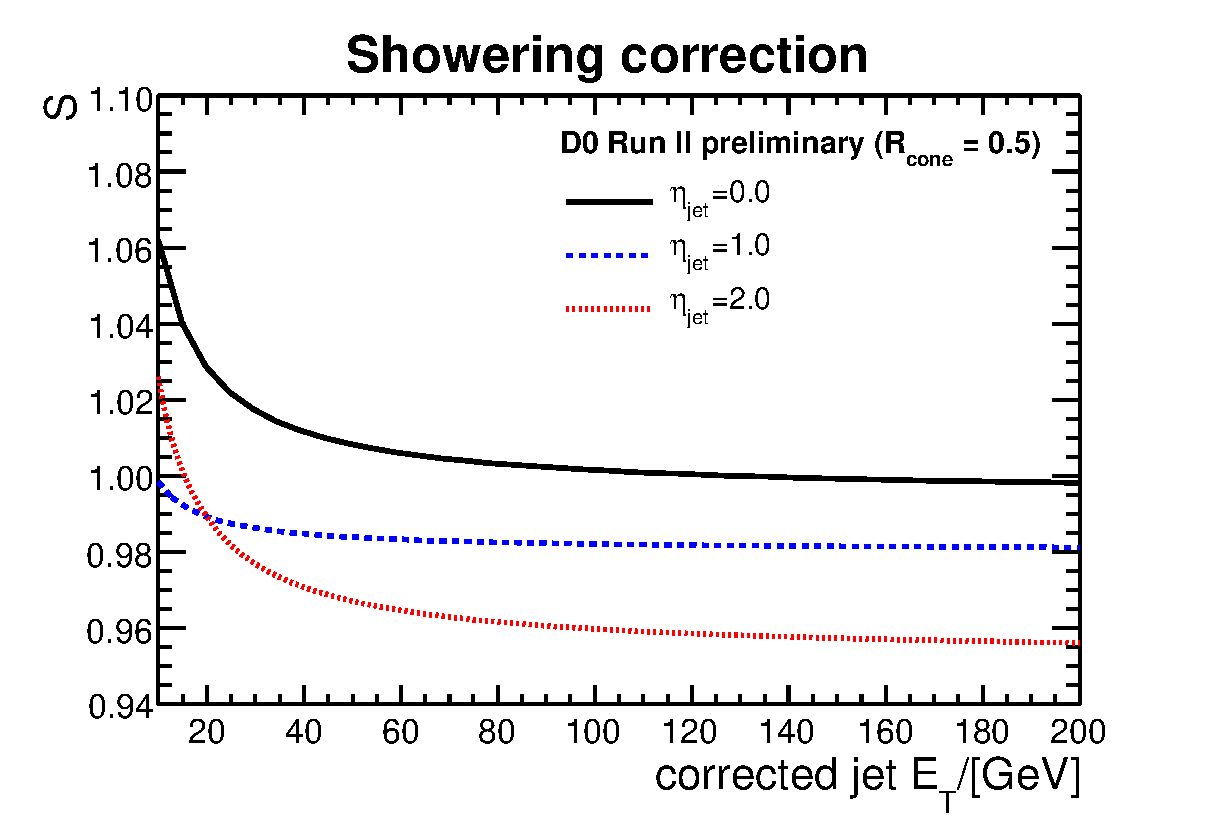
\includegraphics[width=0.75\textwidth]{eps/Reco/JES-shower.eps}
\end{center}
\vspace{-0.1in}
\caption{Showering correction for jets as a function of E$_{T}$ for jets in three different $\eta$ regions~\cite{jes}.}
\label{jes-shower}
\end{figure}

\end{itemize}

\subsection{Missing $E_{T}$}
\label{metreco}

Missing transverse energy is a useful quantity to calculate because it is highly correlated with the transverse energy of the undetected neutrino. The missing energy is only calculated in the transverse plane (x-y) because there is no net momentum in this plane since the proton-antiproton collision only occurs along the beam axis (z)\footnote{The total missing energy of the event can not be calculated because of the unknown boost along the longitudinal direction from the hard scatter process.}.  The missing $E_{T}$ (M$E_{T}$) is defined as the vector sum of the electromagnetic and fine hadronic calorimeter cell energies as well as any lepton $p_{T}$ subtracted from zero such that there is no net transverse momentum in the event. This definition is summarized in Eq.~\ref{met}.

\begin{equation}
\label{met}
\rm{M}E_{T} = -\left[~\sum_{\rm{cells}} E_{T}~\right] - p_{T}(\ell)
\end{equation}

\subsection{$B$-Jets}
\label{bidreco}

$B$-jets are a subset of all jets found by the jet cone algorithm with the distinction that these jets are formed from the hadronization of a $b$ quark. $B$-jets are important to measure because many fundamental particles, such as the top quark, will decay into a $b$ quark leaving it as one of the few signatures of its existence. $B$-jets are unique from jets produced from light quarks because the $B$~hadron (a bound state of a $b$ quark and one or two light quarks) has a much longer lifetime than lighter hadrons. The result of this long lifetime is a displaced decay vertex from the primary interaction vertex. The typical decay length, which is the distance from the decay vertex to the primary vertex, is a few millimeters. The goal of a $B$-jet finding algorithm is to use this property and other kinematically unique characteristics to identify heavy flavor jets from light flavor jets.

The $B$-jet selection algorithm at $\dzero$~uses a neural network (NN) to distinguish heavy flavor jets from light flavor jets~\cite{bid}. The neural network is trained using seven variables that show discrimination between heavy and light flavor jets. The seven variables are shown in Table~\ref{nnvars}.  The network was trained with $Z\rightarrow b\bar{b}$ and strongly produced $b\bar{b}$ production as heavy flavor signal-like events and $Z\rightarrow q\bar{q}$ and strongly produced $q\bar{q}$ production as light flavor background-like events. The output of the neural network is a new variable which peaks at 1 for heavy flavor jets and 0 for light flavor jets. A jet is ``tagged" as a $B$-jet if the NN value is greater than 0.775. Only jets with at least two tracks with $p_{T}>1$~GeV are considered for heavy flavor tagging. Jets which fail this criteria are considered light flavor jets.

\begin{table}[!h!tbp]
\begin{center}
\caption{Variables used in the neural networks training. The variables are listed in order of relative importance as determined in the training~\cite{bid}.}
\label{nnvars}
\begin{tabular}{c|c}
%\multicolumn{2}{c}
%{\underline{Variables Used in $B$-jet Neural Network}} \\
Rank	&	Variable Description	\\
\hline
1		&	Decay length significance ($\frac{L_{T}}{\delta L_{T}}$) of the displaced vertex	\\
2		&	Weighed combination of the input tracks' impact parameter significance ($\frac{IP}{\delta IP}$)	\\
3		&	Probability that the jet originates from the primary interaction vertex	\\
4		&	$\chi^{2}$/N$_{dof}$ of the displaced vertex fit	\\
5		&	Number of tracks used to reconstruct the displaced vertex	\\
6		&	Mass of the tracks used to reconstruct the displaced vertex	\\
7		&	Number of displaced vertices found inside the input jets		\\
\end{tabular}
\vspace{-0.1 in}
\end{center}
\end{table} 

%------------------------------------


\section{Monte Carlo Generation and Detector Simulation}
\label{simulation}

Generating Monte Carlo events is crucial in a physics analysis to understand the signature a given process will have in the detector. The chain for generating simulated Monte Carlo events at $\dzero$ is the following: (1) generate final state four-vectors using Monte Carlo software, (2) simulate the $\dzero$~detector response to final state particles, (3) add additional $\ppbar$~interactions, and finally (4) reconstruct the event. The $\dzero$~trigger simulation is performed separately and described in Section~\ref{triggersim}. The result of the Monte Carlo generation with full detector simulation is a set of events that can be treated as equal to reconstructed data except with a known initial hard scatter physics process.

The first stage of generating Monte Carlo events is to produce and decay particles according to a specified physics process. The hard scatter collision is typically generated by ``matrix-element" generators, such as CompHEP or Alpgen, and the decay products are typically handled by particle-specific algorithms. Specifically, the decay of tau leptons is handled by TAUOLA~\cite{1993CoPhC..76..361J} and B hadrons are decayed by EVTGEN~\cite{2001NIMPA.462..152L}. To simulate hardronization and allow for additional strong interaction effects between final state particles, all Monte Carlo events are processed through the Pythia generator.

The $\dzero$~detector is simulated using the GEANT software package~\cite{geant}. GEANT\footnote{GEANT is an acronym formed from "GEometry ANd Tracking".} provides a graphical representation of particles as they traverse the detector and simulates the interaction between particles and material in the detector. All information concerning the detector geometry and material density is modeled with GEANT. Three examples of GEANT's capabilities are simulating electromagnetic and hadronic showers in the calorimeter, energy loss of electrons in the tracking detector, and bending particle trajectories due to the solenoidal and toroidal magnetic fields.

To properly account for additional inelastic $\ppbar$~collisions all Monte Carlo events are provided with a ``minimum bias overlay" generated from reconstructed data. A minimum bias event is an event recorded by the detector that was triggered solely by the presence of at least one $\ppbar$~interaction. Because the number of minimum bias vertices grows with instantaneous luminosity the minimum bias events are overlaid to match the expected instantaneous luminosity profile of all recorded events. A plot of the average peak instantaneous luminosity versus time is shown in Fig.~\ref{peaklumi}.

\begin{figure}[!h!tbp]
\begin{center}
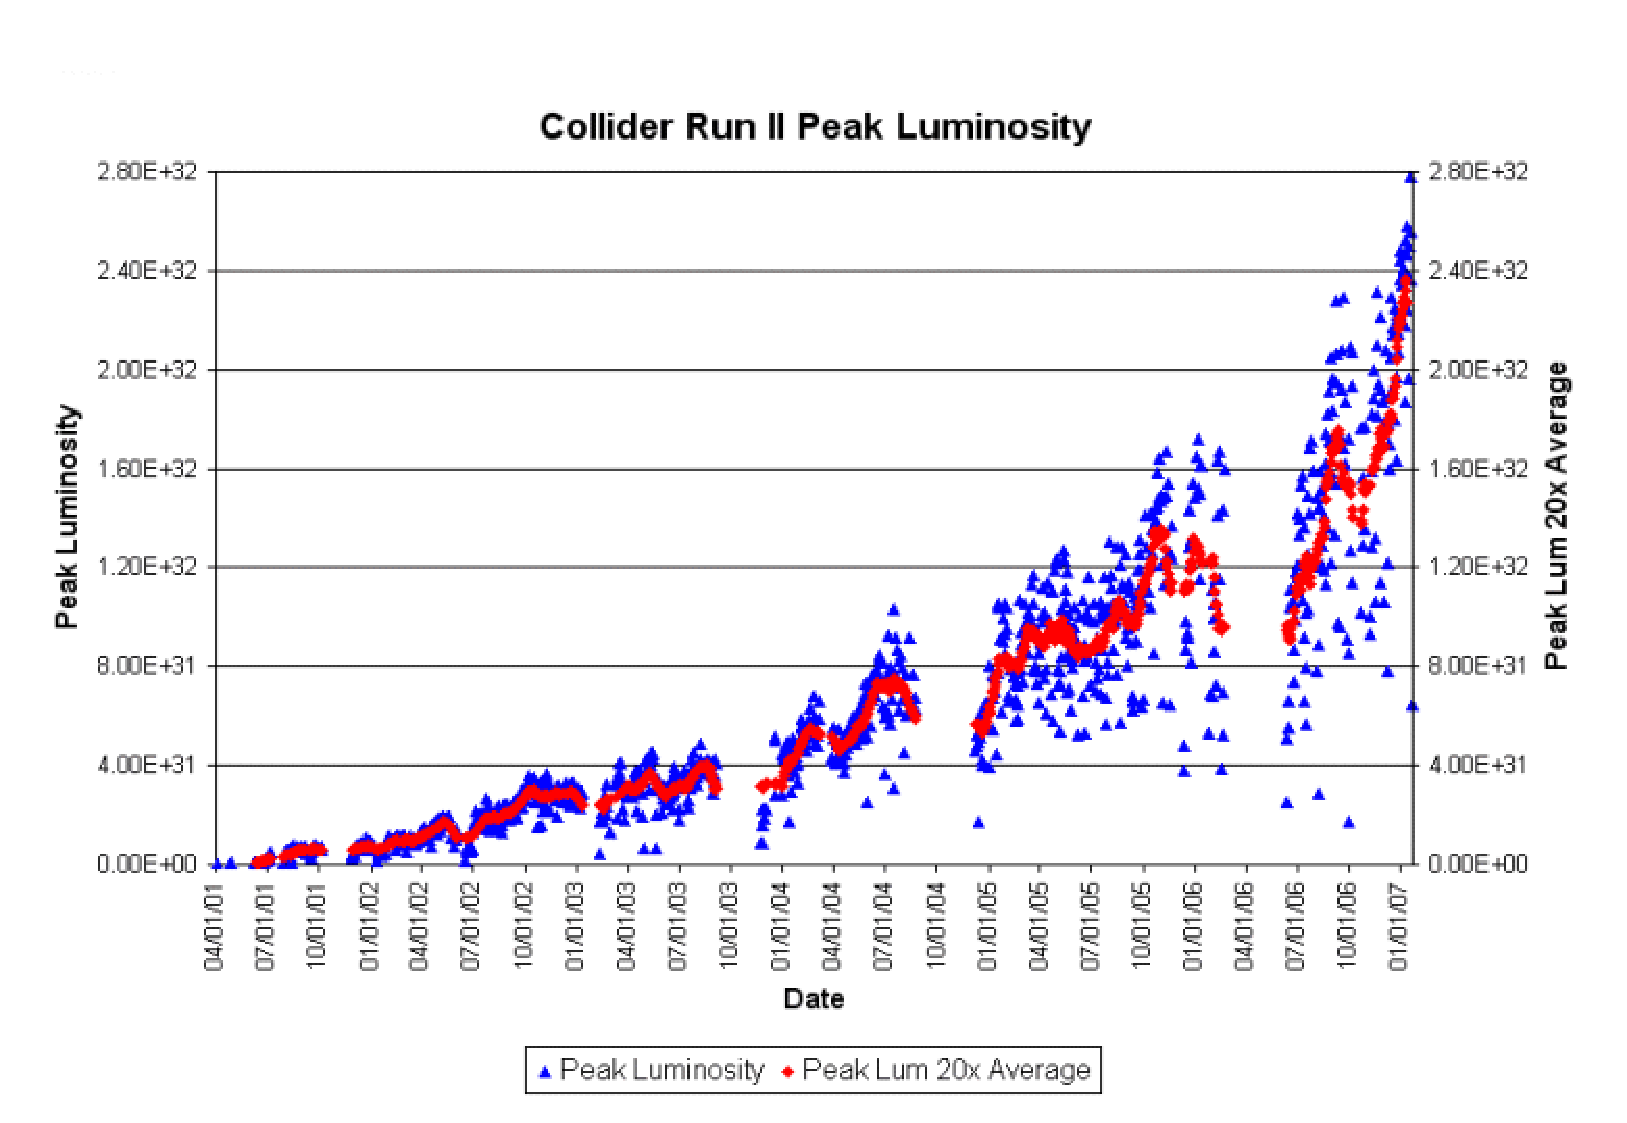
\includegraphics[width=0.75\textwidth]{eps/Reco/InstanteousLuminosity.eps}
\end{center}
\vspace{-0.1in}
\caption{Peak instantaneous luminosity as a function of time~\cite{tevlumi}.}
\label{peaklumi}
\end{figure}

Reconstruction of Monte Carlo events occurs in the same manner as data events, as described in Section~\ref{objectreco}. It is the goal of the previous three steps of the simulation chain to describe the $\dzero$~detector response as accurately as possible such that the reconstruction is blind to the source of the event.

\section{Trigger Simulation}
\label{triggersim}

The $\dzero$~trigger system is modeled in a Monte Carlo event by an event-wide probability that the event will pass the trigger selection. The event-wide probability is constructed from the efficiencies with which individual reconstructed objects pass object specific ``trigger terms". Section~\ref{triggerprob} derives the event-wide trigger probability in terms of individual trigger term efficiencies and Section~\ref{triggereffmethod} describes the methods used to measure these efficiencies. Triggers used to record single top quark events and their efficiencies are shown in Chapter~\ref{analysis}.

\subsection{Event-Wide Trigger Probability}
\label{triggerprob}

The probability that a Monte Carlo event $\vec{x}$ is selected by the trigger is defined as a product of the condition probabilities to pass each trigger level given that it passed the previous trigger level as shown in Eq.~\ref{trigprob}.

\begin{equation}
\label{trigprob}
P_{\rm{Trigger}}(\vec{x}) = \left[ \prod_{\rm{Terms}}P_{\rm{L1}}(\vec{x}) \right ] \times \left[ \prod_{\rm{Terms}}P_{\rm{L2|L1}}(\vec{x}) \right ] \times \left[ \prod_{\rm{Terms}}P_{\rm{L3|L2}}(\vec{x}) \right ]
\end{equation}

At a given trigger level the probability for the event to be selected is written as the product of each reconstructed object to be selected by each trigger term as shown in Eq.~\ref{triglevelprob}. For example, the probability for a muon+2~jet event to pass a $\mu$+jets trigger is the product of the probability for the muon to pass the muon trigger term and the two jets to pass the jet trigger term.

\begin{equation}
\label{triglevelprob}
P_{\rm{Level}}(\vec{x}) = \prod_{k}^{\rm{Nobs}} P_{\rm{Level,Object}}(\vec{x}_{\rm{Object}})
\end{equation}

The probability for a reconstructed object to pass a certain trigger level is written as one minus the probability of all the objects not to be selected by the trigger, as shown in Eq.~\ref{triglevelprobobject}

\begin{equation}
\label{triglevelprobobject}
P_{\rm{Level,Object}}(\vec{x}_{\rm{Object}}) = 1 - \prod_{j}^{\rm{Nobjs}}( 1 - \varepsilon_{\rm{Level}}(\vec{x}_{\rm{Object},j}) )
\end{equation}

\noindent where $\varepsilon_{\rm{Level}}(\vec{x}_{\rm{Object},j})$~is the trigger term efficiency for the reconstructed object.

At $\dzero$ there have been several distinct trigger periods where the trigger used to collect data events has changed. To model this in Monte Carlo an integrated luminosity weighted average of the trigger probabilities for each period is applied to all events. The weighted averaged is shown in Eq.~\ref{triggerweight}

\begin{equation}
\label{triggerweight}
P(\vec{x}) = \frac{\sum_{\rm{version}} \left[ \mathcal{L}_{\rm{version}} \times P_{\rm{version}}(\vec{x}) \right]}{\sum_{\rm{version}} \mathcal{L}_{\rm{version}}}
\end{equation}

\subsection{Trigger Term Efficiency Measurement Methods}
\label{triggereffmethod}

Electron and muon trigger term efficiencies are measured in $Z\rightarrow ee$ and $Z\rightarrow \mu\mu$ data events, respectively. The efficiency is measured in a $Z$ boson sample because it provides a clean (i.e. negligible background) sample of leptons with which to measure efficiencies. In the $Z$ sample a ``tag and probe" method is used to measure the trigger efficiency where one of the leptons is required to trigger the event such that the other can be used as an unbiased probe to measure the trigger efficiency. The efficiency is defined as the fraction of events for which the probe electron or muon was found to pass the trigger term. To account for detector and reconstruction effects the trigger efficiencies are determined as a function of $p_{T}$, $\eta$, or $\phi$. An example of the L1 muon trigger efficiency and the L3 electron trigger efficiency binned in $\eta$ and $p_{T}$ are shown in Fig.~\ref{triggereffexample}. Jet trigger term efficiencies are measured in muon triggered events. The jet trigger efficiency is defined as the number of jets that pass the jet trigger term divided by the total number of jets. Jet trigger term efficiencies are measured as a function of $p_{T}$ and $\eta$.


\begin{figure}[!h!tbp]
\begin{center}
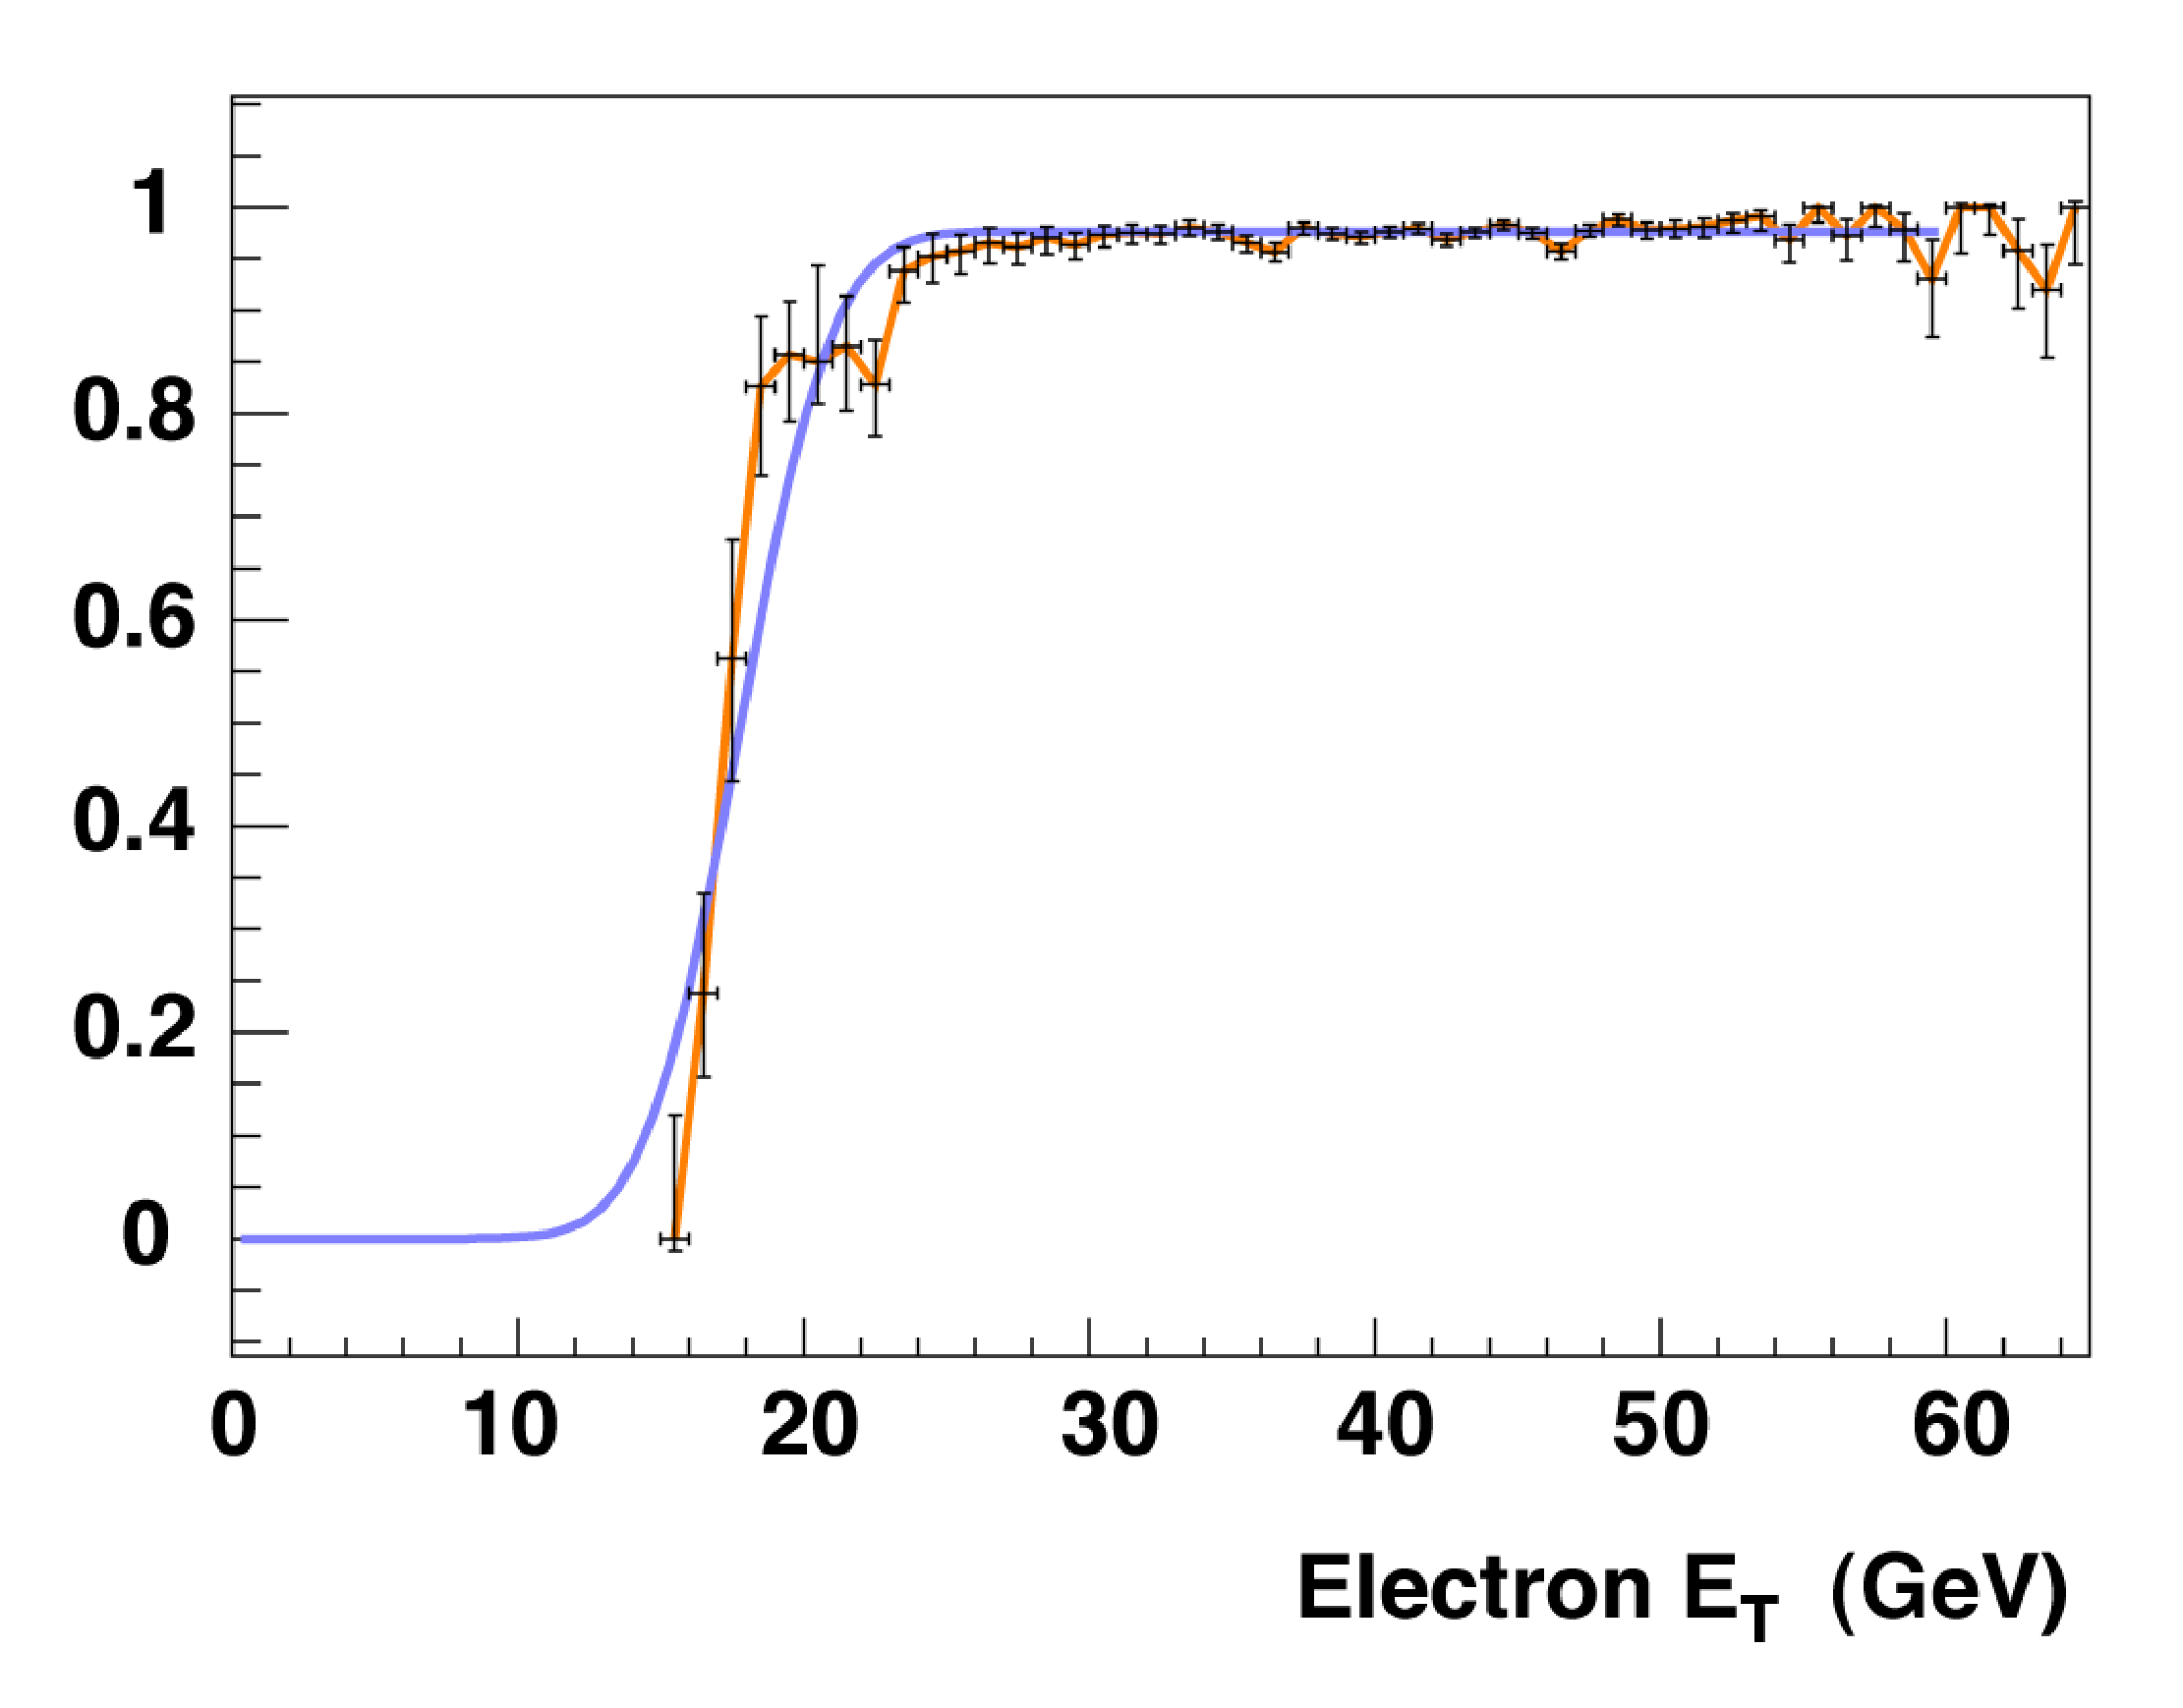
\includegraphics[width=0.49\textwidth]{eps/Reco/electron_turn-on_curve_pt.eps}
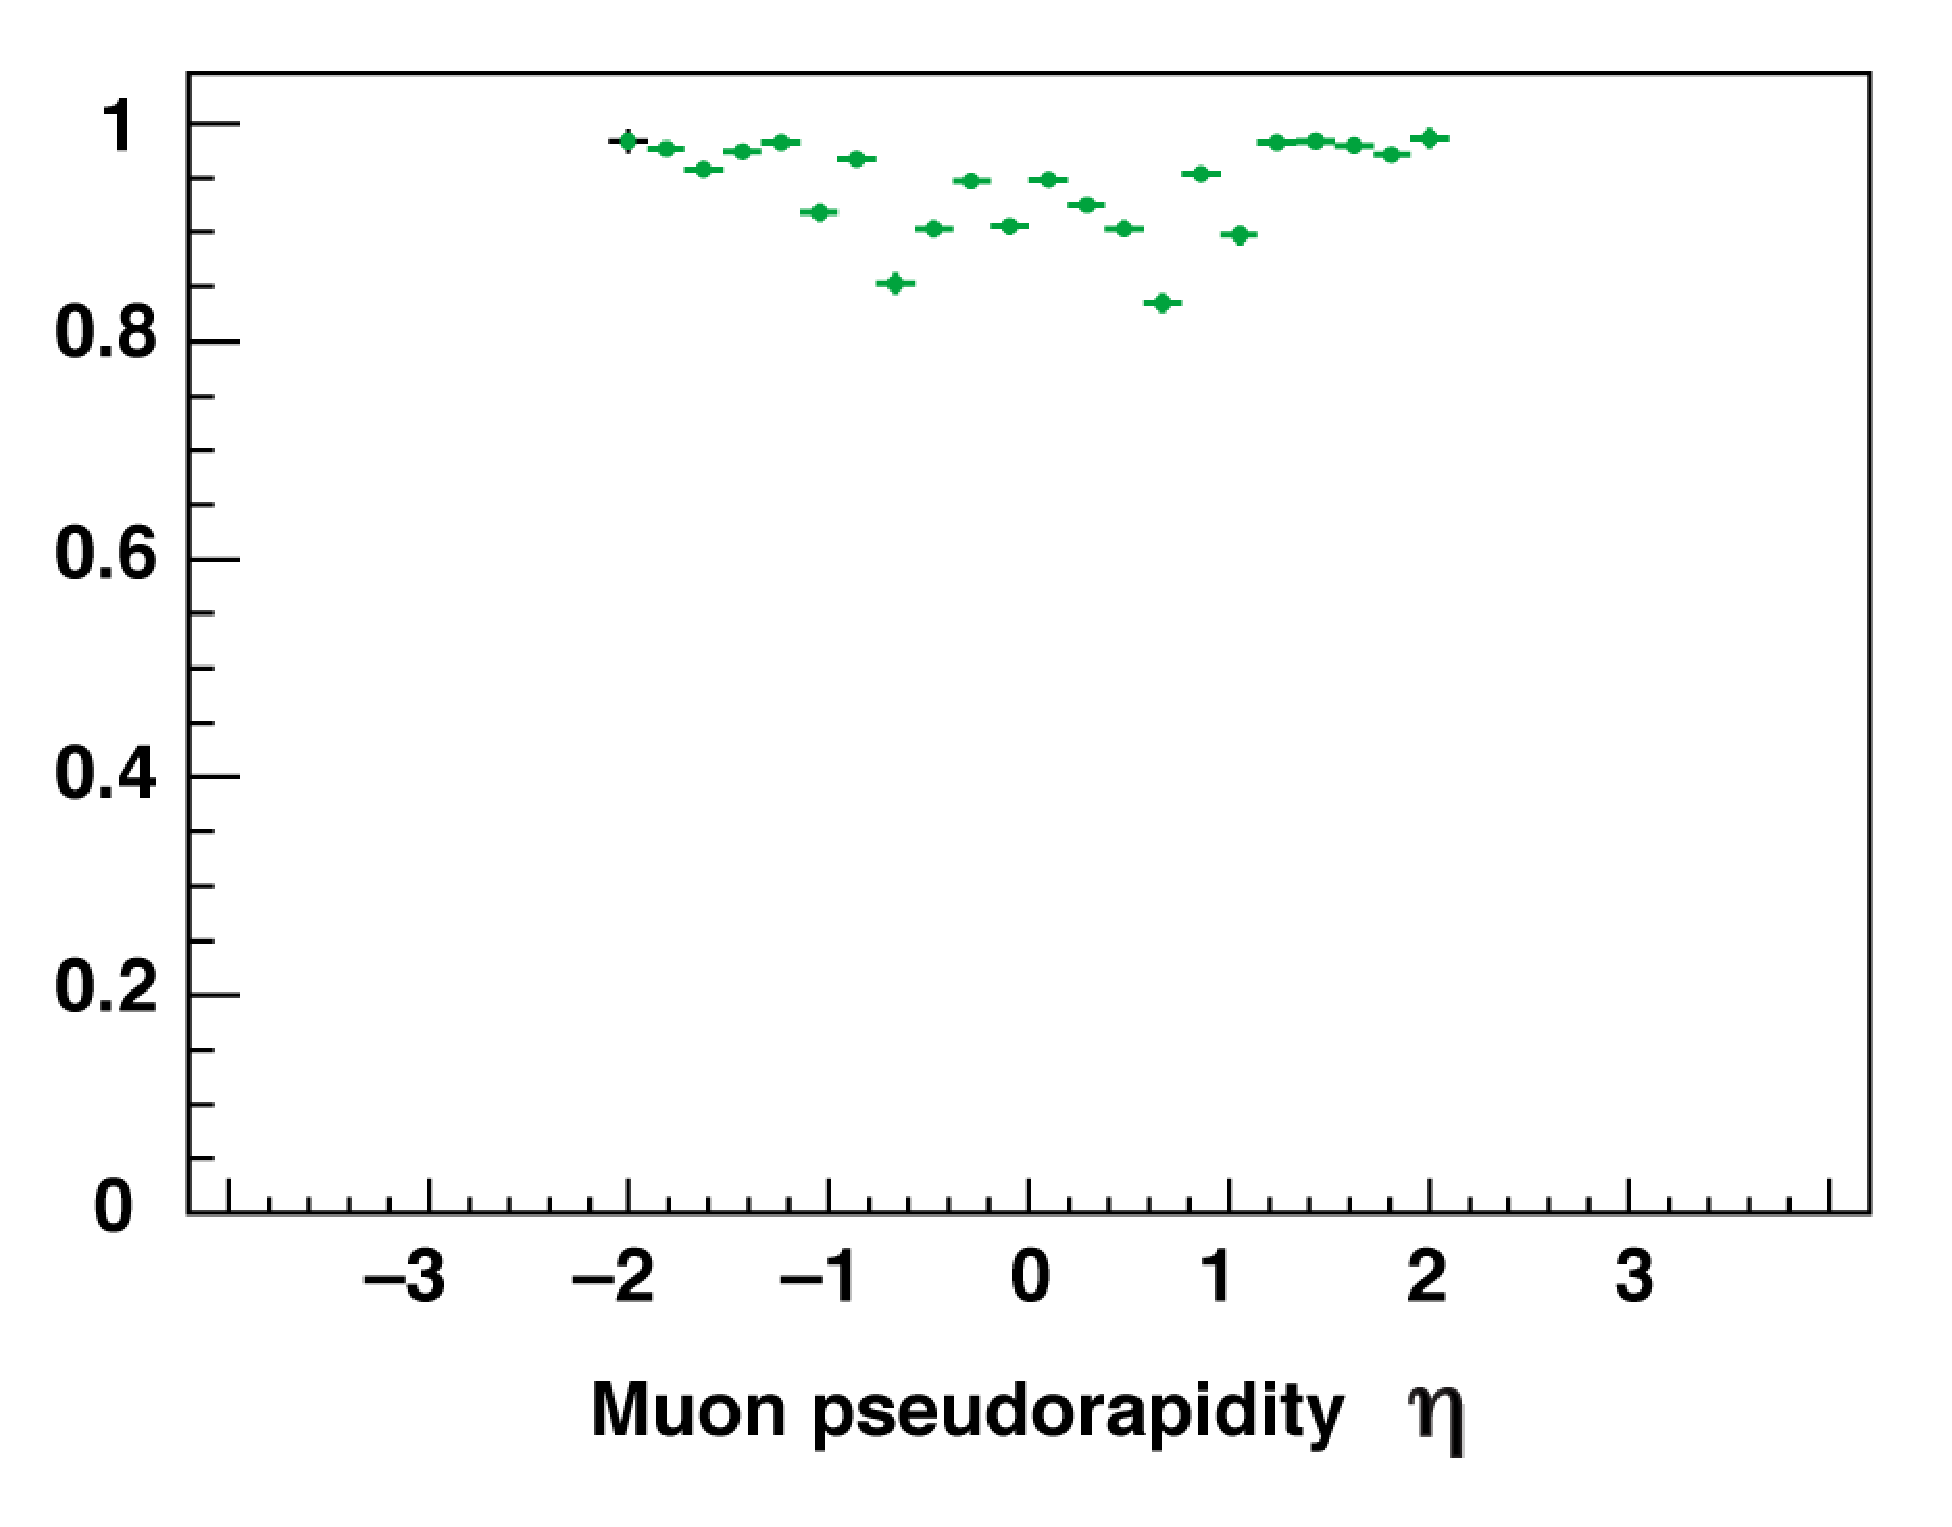
\includegraphics[width=0.49\textwidth]{eps/Reco/muon_turn-on_curve_eta.eps}
\end{center}
\vspace{-0.1in}
\caption{An example electron turn-on curve measured
as a function of the electron $p_{T}$ (left) and
an example muon turn-on curve measured as a function of $\eta$ (right). The points are trigger efficiencies derived from data
in that bin (with uncertainty bars)~\cite{singletopnote}.}
\label{triggereffexample}
\end{figure}


\section{Monte Carlo Corrections}
\label{corrections}

The result of the Monte Carlo generation with a full detector simulation are events that mimic real data events recorded by the $\dzero$~detector. Typically, however, the simulation is not complete for reasons such as missing material in the GEANT simulation or un-modeled aging effects of the detector. The result of not modeling these effects typically leads to an overestimation of detector resolution in the Monte Carlo. To account for this the reconstructed Monte Carlo objects are typically ``smeared" in one variable to ensure similar resolutions as is seen in data events. After the Monte Carlo events are smeared the relative difference between Monte Carlo and data events is measured and used to further correct the Monte Carlo. The following sections describe the smearing and correction factors for all reconstructed objects.


\subsection{Muons}

Muon smearing and correction factors are measured in $Z\rightarrow \mu\mu$ events because it provides a clean and unbiased sample of muons in both data and Monte Carlo. While the presence of a muon is confirmed by hits in the muon system the muon momentum vector is defined by the matched track. The muon track is defined by the charge and radius of curvature, which is proportional to $q/p_{T}$, thus the natural quantity to smear is $q/p_{T}$. The amount to which the muon track must be smeared is measured by observing the relative shift and width of the $Z$ boson resonance in data and Monte Carlo events. The functional form to which the muon track is smeared is shown in Eq.~\ref{muonsmear}.

\begin{equation}
\label{muonsmear}
\left( \frac{q}{p_{T}} \right)^{'} \rightarrow \frac{q}{p_{T}} + (A + \frac{B}{p_{T}})\times G
\end{equation}

\noindent The parameter $G$ is a random number generated from a Gaussian distribution centered at 0 and a width of 1. The parameters A and B are measured for muons with an SMT track hit in two regions ($\eta<1.6$ and $\eta>1.6$) and for muons without an SMT hit. Table~\ref{muonsmearparam} shows the smearing parameters for the three types of muons for two separate run periods.


\begin{table}[!h!tbp]
\begin{center}
\caption{Muon smearing parameters for the function $(A + \frac{B}{p_{T}})$ for two different run periods.}
\label{muonsmearparam}
\begin{tabular}{c|cc|cc|}
%\multicolumn{5}{c}
%{\underline{Muon Smearing Parameters}} \\
       & \multicolumn{2}{|c|}{$<$~Dec.~2004} & \multicolumn{2}{|c}{$>$~Dec.~2004} \\
Muon Type				&	A		&	B		&	A		&	B		\\
\hline
$>1$ SMT Hit ($\eta<1.6$)	&	0.00313	&	-0.0563	&	0.00308	&	-0.0370	\\
$>1$ SMT Hit ($\eta>1.6$)	&	0.00273	&	-0.0491	&	0.00458	&	-0.0550	\\
$=0$ SMT Hits				&	0.00509	&	-0.0916	&	0.00424	&	-0.0509	\\
\end{tabular}
\vspace{-0.1 in}
\end{center}
\end{table} 


After the smearing is applied the correction factor for muons is defined as the product of three independent factors, as shown in Eq.~\ref{muonscalefactor}, for reconstruction, track matching, and isolation.

\begin{equation}
\label{muonscalefactor}
f_{\rm{Data/MC}}(\mu) = \frac{\varepsilon^{\rm{Data}}_{\rm{Reco}}(\mu)}{\varepsilon^{\rm{MC}}_{\rm{Reco}}(\mu)} \times 
\frac{\varepsilon^{\rm{Data}}_{\rm{Track|Reco}}(\mu)}{\varepsilon^{\rm{MC}}_{\rm{Track|Reco}}(\mu)} \times \frac{\varepsilon^{\rm{Data}}_{\rm{Isolation|Track}}(\mu)}{\varepsilon^{\rm{MC}}_{\rm{Isolation|Track}}(\mu)}
\end{equation}

The muon reconstruction efficiency for data and the Monte Carlo correction factor are shown in Fig.~\ref{muonrecoeffscale}. The empty region in the center of the $\eta$-$\phi$ efficiency histogram corresponds to the hole in the bottom of the muon detector. The correction factor is only considered to be a function of $\eta$ since the reconstruction efficiencies for data and Monte Carlo show the same $\phi$ dependence. The average reconstruction efficiency in data is 80.2$\%$ and the average Monte Carlo correction factor is $0.97$.

\begin{figure}[!h!tbp]
\begin{center}
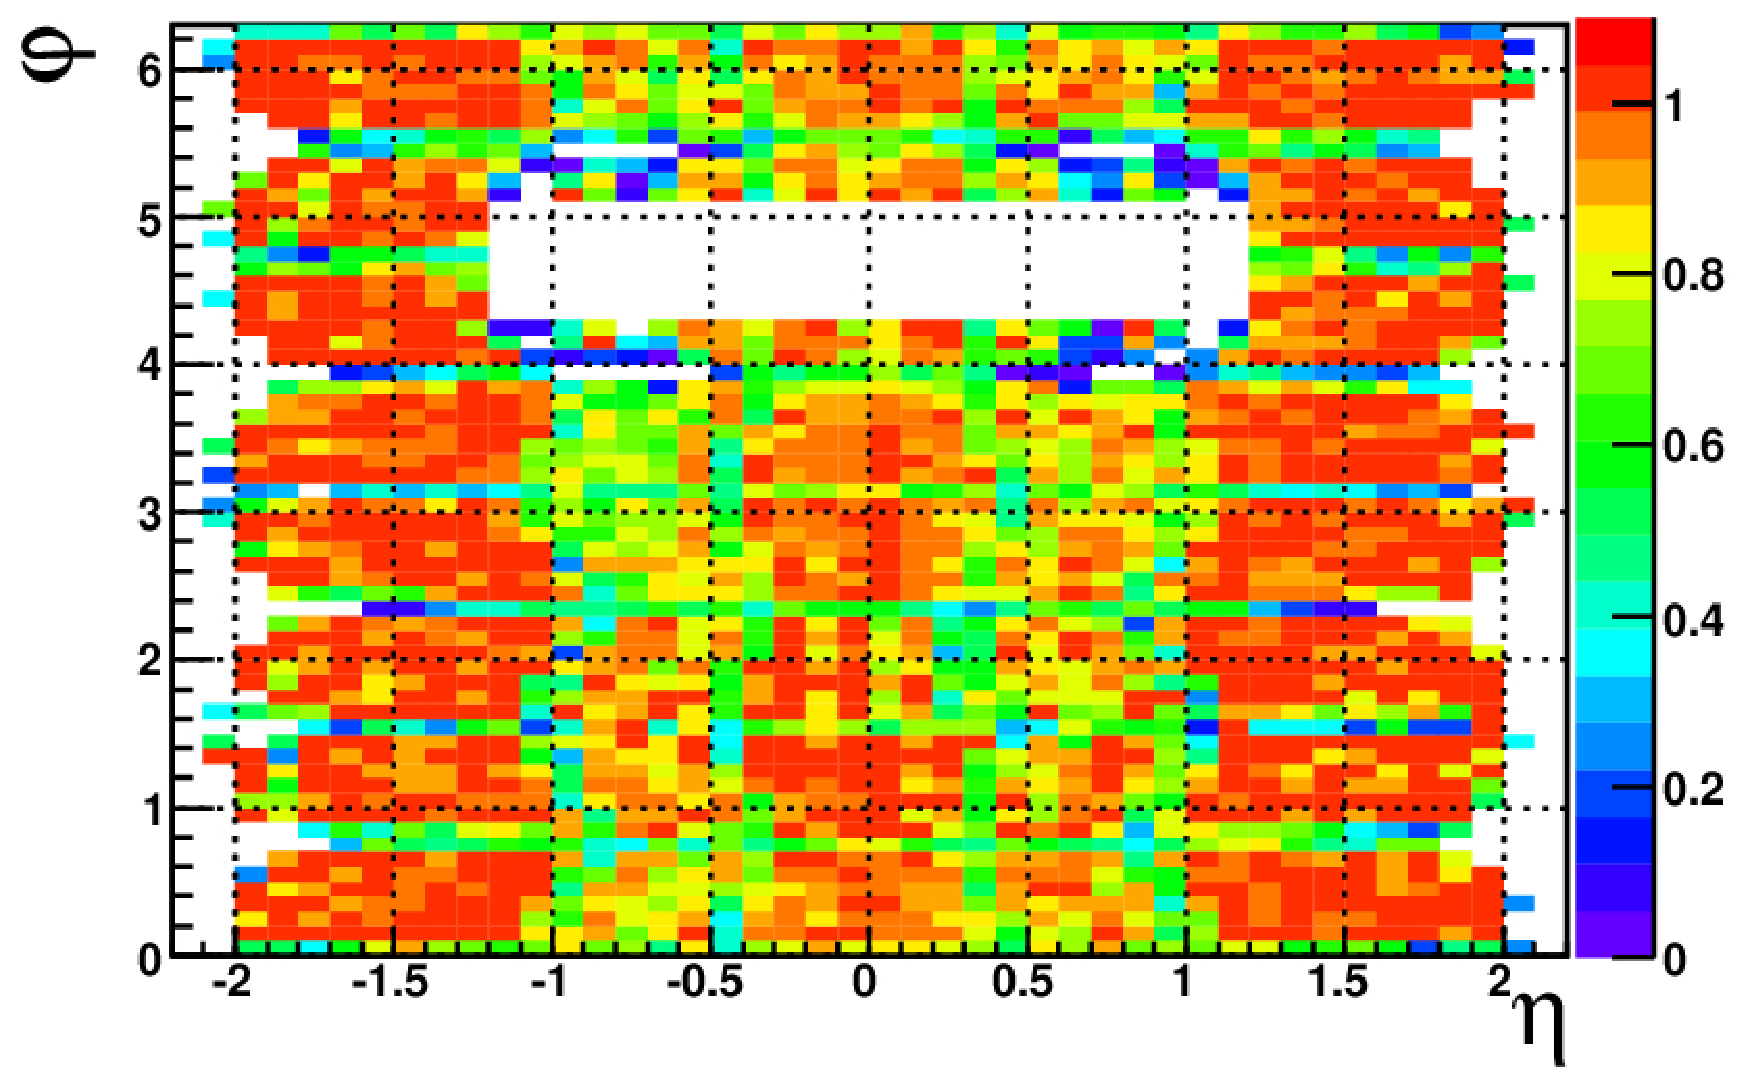
\includegraphics[width=0.49\textwidth]{eps/Reco/muonreco.eps}
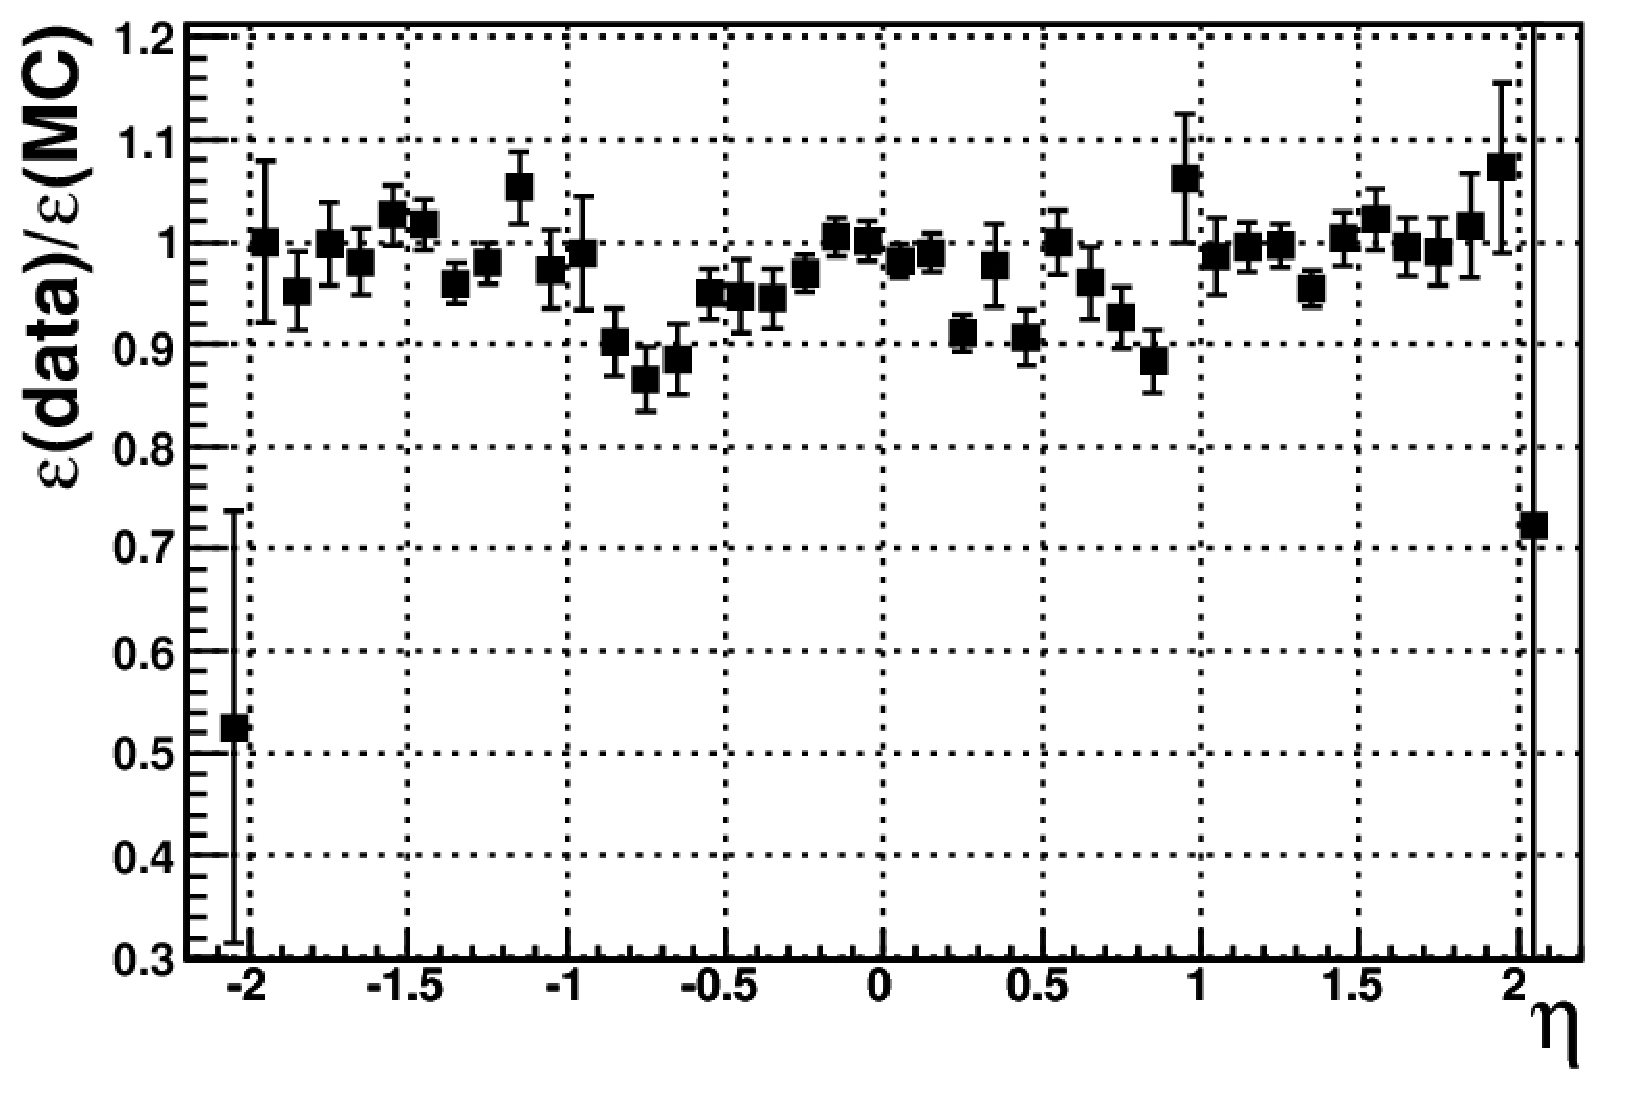
\includegraphics[width=0.49\textwidth]{eps/Reco/muonrecoscale.eps}
\end{center}
\vspace{-0.1in}
\caption{Muon reconstruction efficiency as measured in $Z\rightarrow \mu\mu$ data events (left) and the Monte Carlo correction factor as a function of muon $\eta$ (right)~\cite{muon}.}
\label{muonrecoeffscale}
\end{figure}

The muon track match efficiency is measured with respect to reconstructed muons. The efficiency is found to depend on two tracking related quantities, the track $\eta$ and the longitudinal primary interaction vertex position. The efficiency in data and correction factor are shown in Fig.~\ref{muontrackeffscale}. The average track match efficiency in data is 91.0$\%$ and the average Monte Carlo correction factor is $0.93$.

\begin{figure}[!h!tbp]
\begin{center}
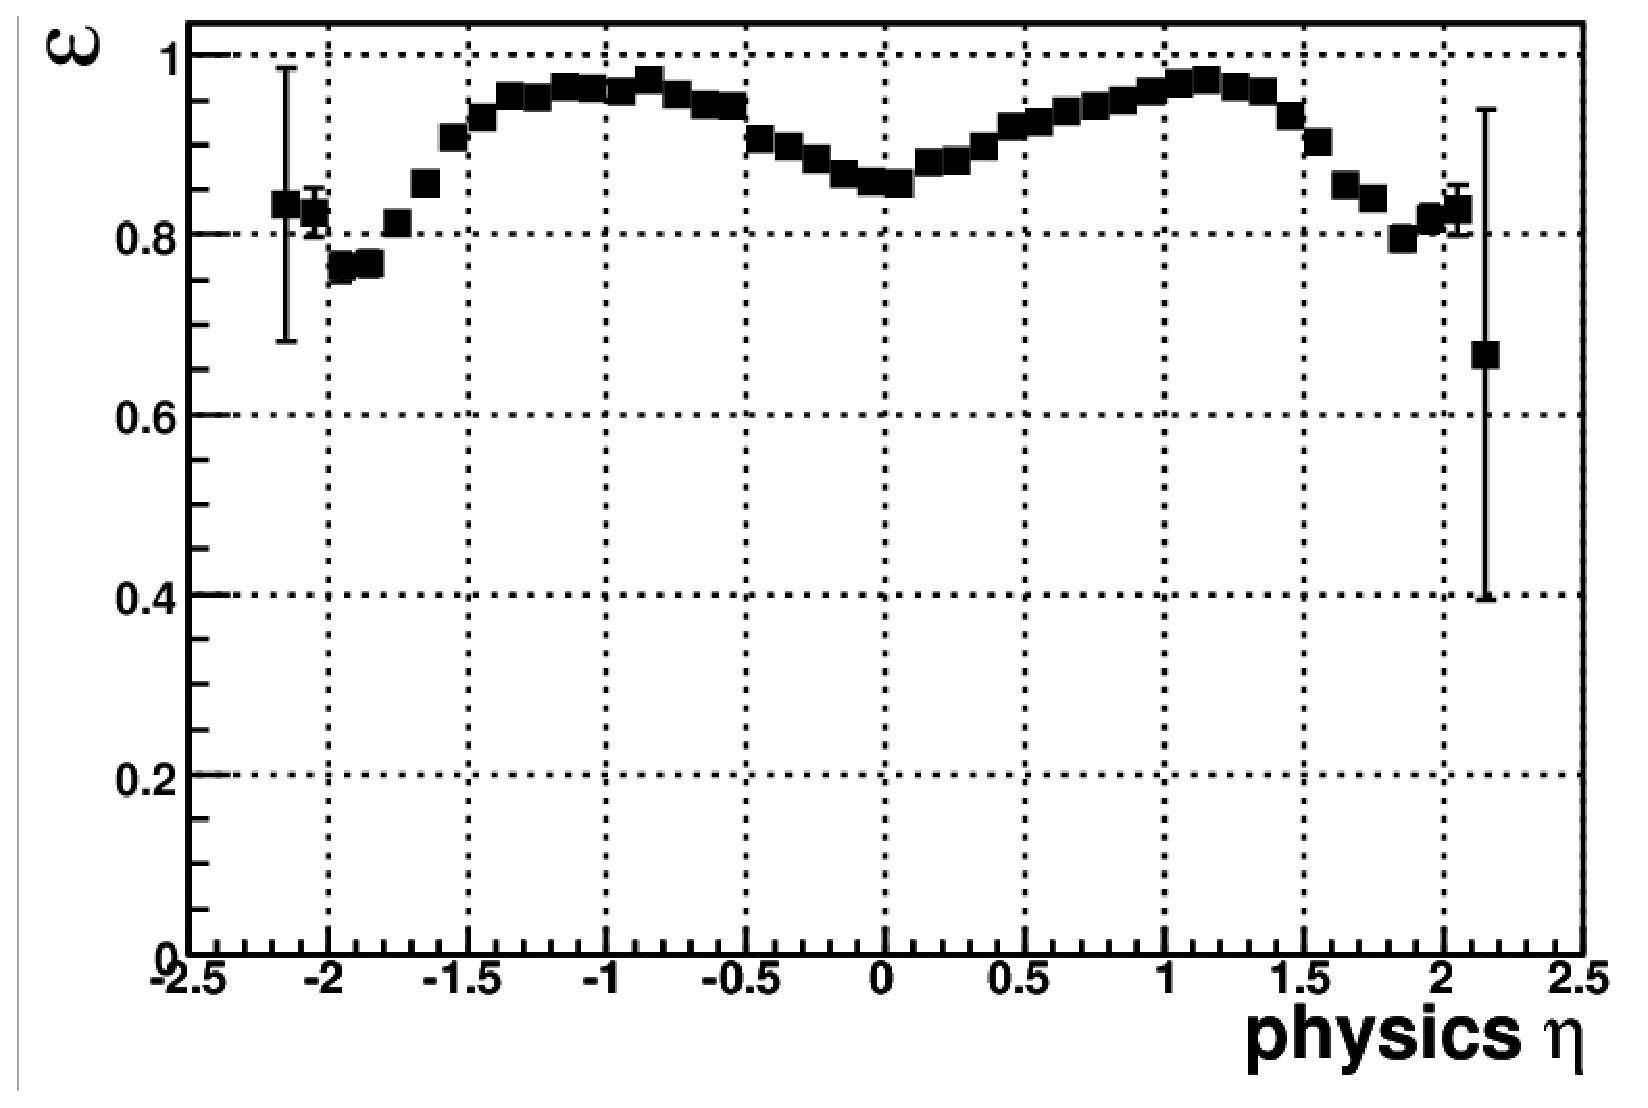
\includegraphics[width=0.49\textwidth]{eps/Reco/muontrack.eps}
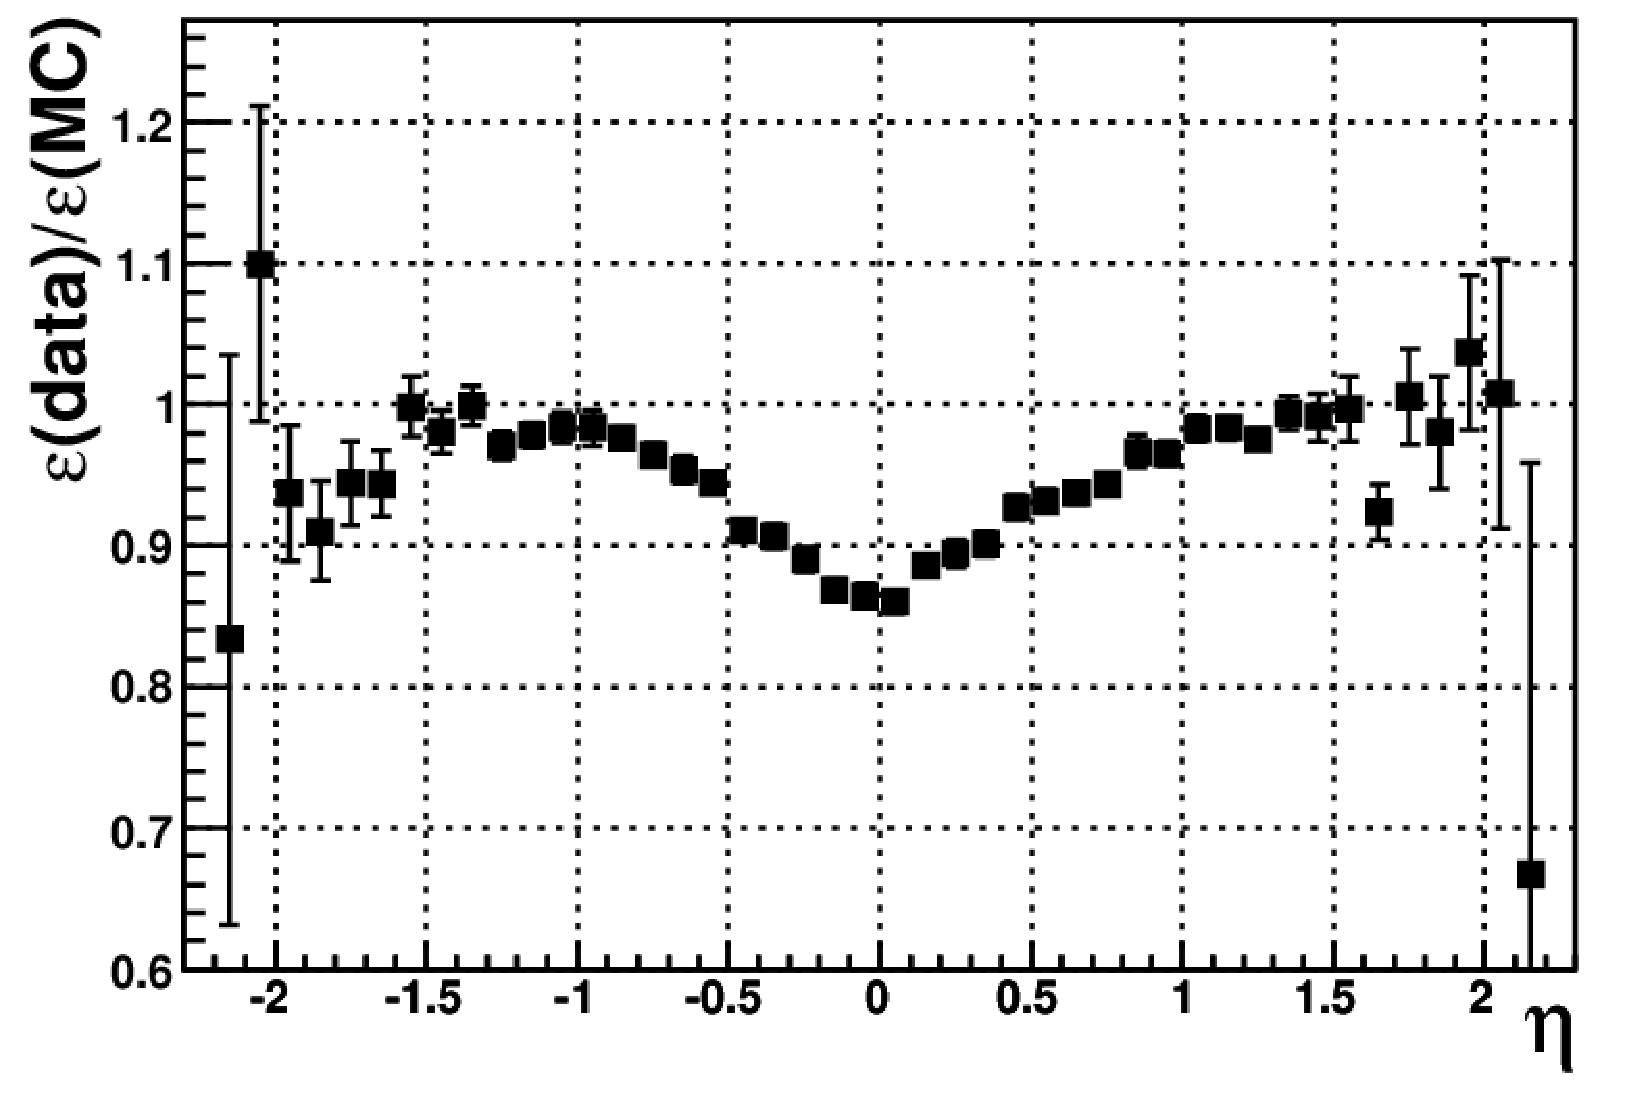
\includegraphics[width=0.49\textwidth]{eps/Reco/muontrackscale.eps}
\end{center}
\vspace{-0.1in}
\caption{Muon track match efficiency as measured in $Z\rightarrow \mu\mu$ data events (left) and the Monte Carlo correction factor as a function of track $\eta$ (right)~\cite{muon}.}
\label{muontrackeffscale}
\end{figure}

The muon isolation efficiency is measured in $Z\rightarrow\mu\mu$ events for reconstructed muon with a confirmed track match. The isolation efficiency depends most strongly on the number of reconstructed jets in the event since it is more difficult for a muon to be isolated if the jets occupy more space in the detector. Fig.~\ref{muonisoeffscale} shows the isolation efficiency and Monte Carlo correction factor as a function of the jet multiplicity. The Monte Carlo correction factor for events with two or three jets, such as single top quark events, is $0.98$, with an average efficiency of $0.94\%$.

\begin{figure}[!h!tbp]
\begin{center}
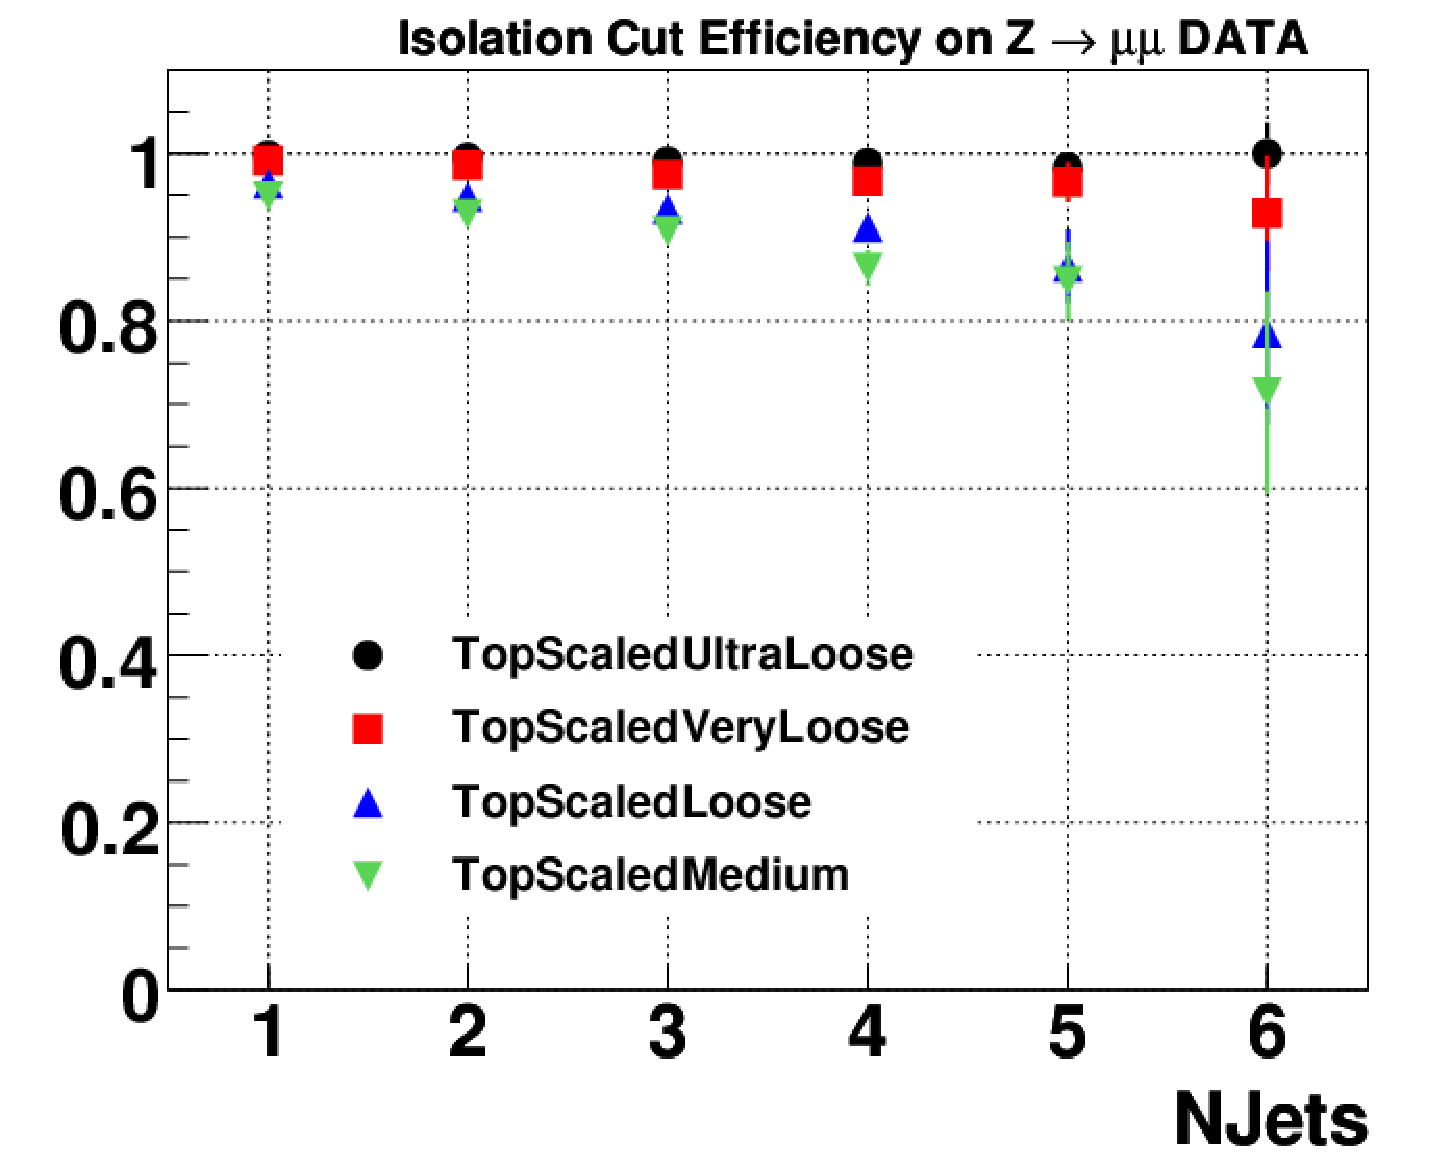
\includegraphics[width=0.49\textwidth]{eps/Reco/muoniso.eps}
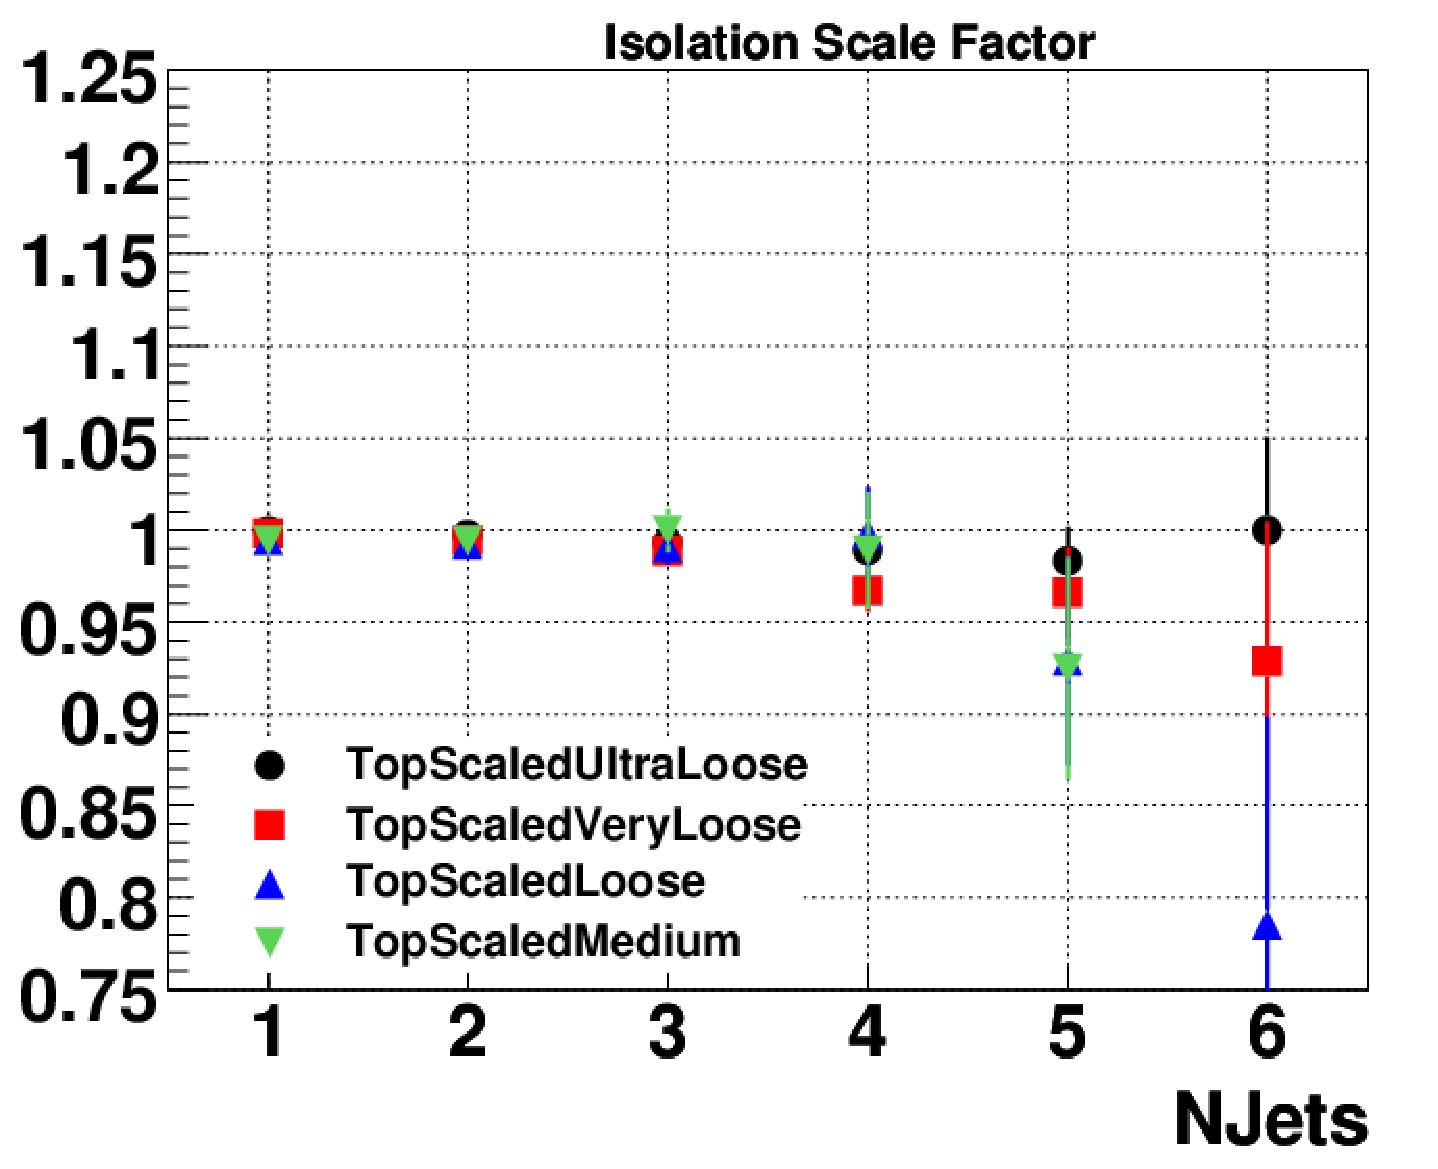
\includegraphics[width=0.49\textwidth]{eps/Reco/muonisoscale.eps}
\end{center}
\vspace{-0.1in}
\caption{Muon isolation efficiency as measured in $Z\rightarrow \mu\mu$ data events for various regions of primary vertex $z$ position (left) and Monte Carlo correction factor as a function of the number of reconstructed jets. The isolation used in the single top quark analysis is labeled TopScaledLoose and corresponds to the blue triangle curve~\cite{muon}.}
\label{muonisoeffscale}
\end{figure}


\subsection{Electrons}

There is no smearing applied to Monte Carlo electrons since the resolution is well-modeled in the Monte Carlo. Electron correction factors are measured in $Z\rightarrow ee$ data and Monte Carlo events. The correction factor for electrons is considered a product of two independent factors: reconstruction and track match plus likelihood cuts, as shown in Eq.~\ref{electronscalefactor}.

\begin{equation}
\label{electronscalefactor}
f_{\rm{Data/MC}}(e) = \frac{\varepsilon^{\rm{Data}}_{\rm{Reco}}(e)}{\varepsilon^{\rm{MC}}_{\rm{Reco}}(e)} \times 
\frac{\varepsilon^{\rm{Data}}_{\rm{TrackMatchLikelihood|Reco}}(e)}{\varepsilon^{\rm{MC}}_{\rm{TrachMatchLikelihood|Reco}}(e)}
\end{equation}

Electron reconstruction efficiencies as measured in $Z\rightarrow ee$ data and Monte Carlo events and the Monte Carlo correction factor show a slight $p_{T}$ dependence as seen in Fig.~\ref{electronrecoeffscale}.

\begin{figure}[!h!tbp]
\begin{center}
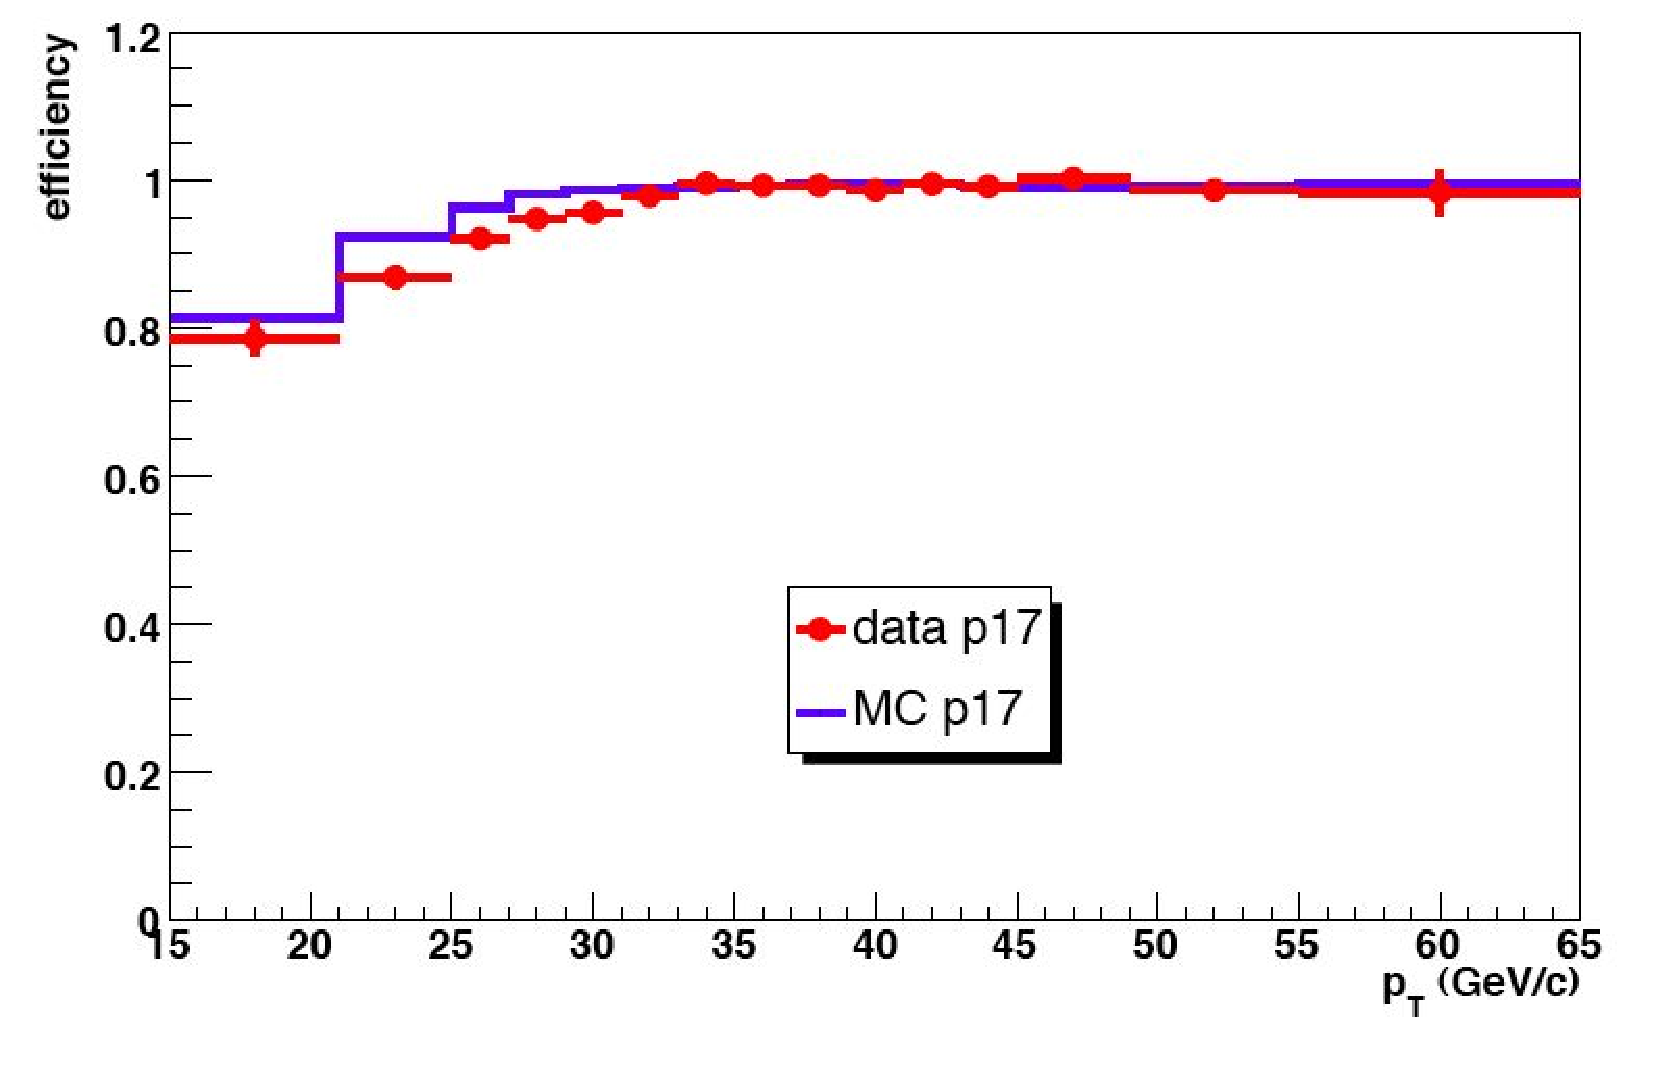
\includegraphics[width=0.49\textwidth]{eps/Reco/Electron_Reco_eff.eps}
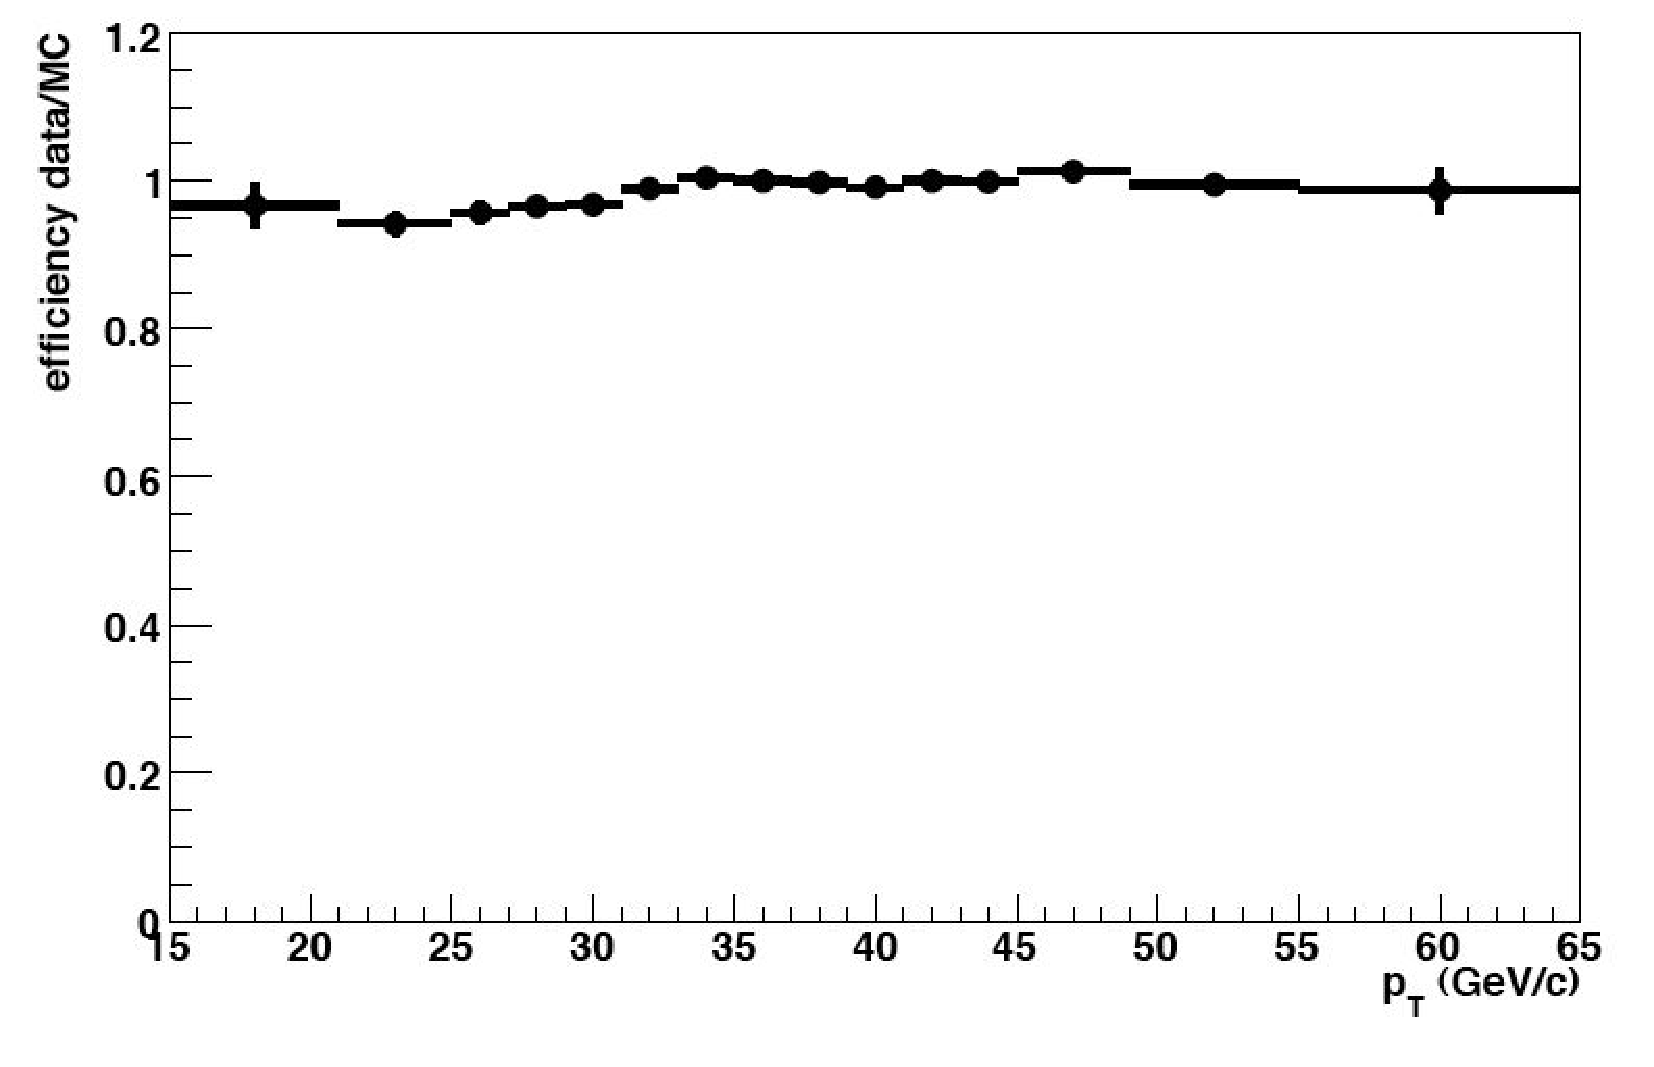
\includegraphics[width=0.49\textwidth]{eps/Reco/Electron_Reco_scale.eps}
\end{center}
\vspace{-0.1in}
\caption{Electron reconstruction efficiency as measured in $Z\rightarrow ee$ data (red) and Monte Carlo (blue) events (left) and Monte Carlo correction factor as a function of electron $p_{T}$ (right)~\cite{electron}.}
\label{electronrecoeffscale}
\end{figure}

Electron likelihood and track match efficiencies are measured in $Z\rightarrow ee$ data and Monte Carlo events with respect to reconstructed electrons. The efficiency in data and the Monte Carlo correction factor are shown in Fig.~\ref{electronlikelihoodeffscale}. The single top quark analysis only use electrons out to 1.1 in $\eta^{det}$.

\begin{figure}[!h!tbp]
\begin{center}
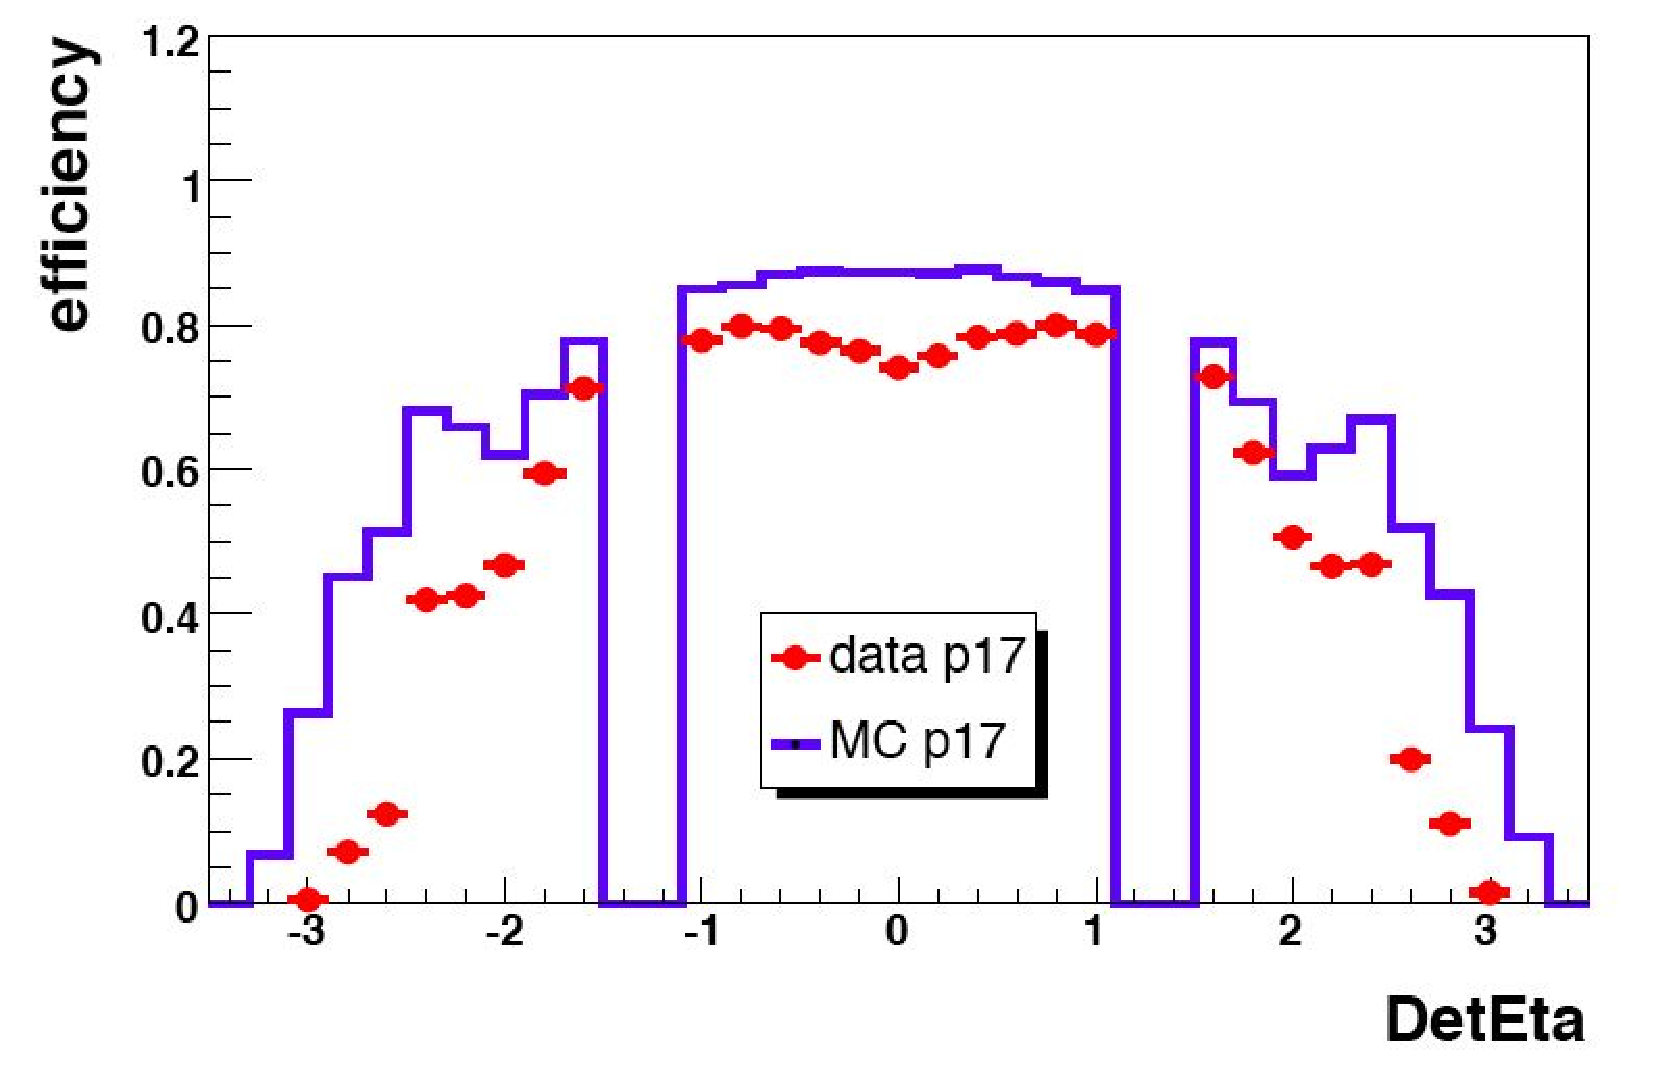
\includegraphics[width=0.49\textwidth]{eps/Reco/Electron_Likelihood_eff.eps}
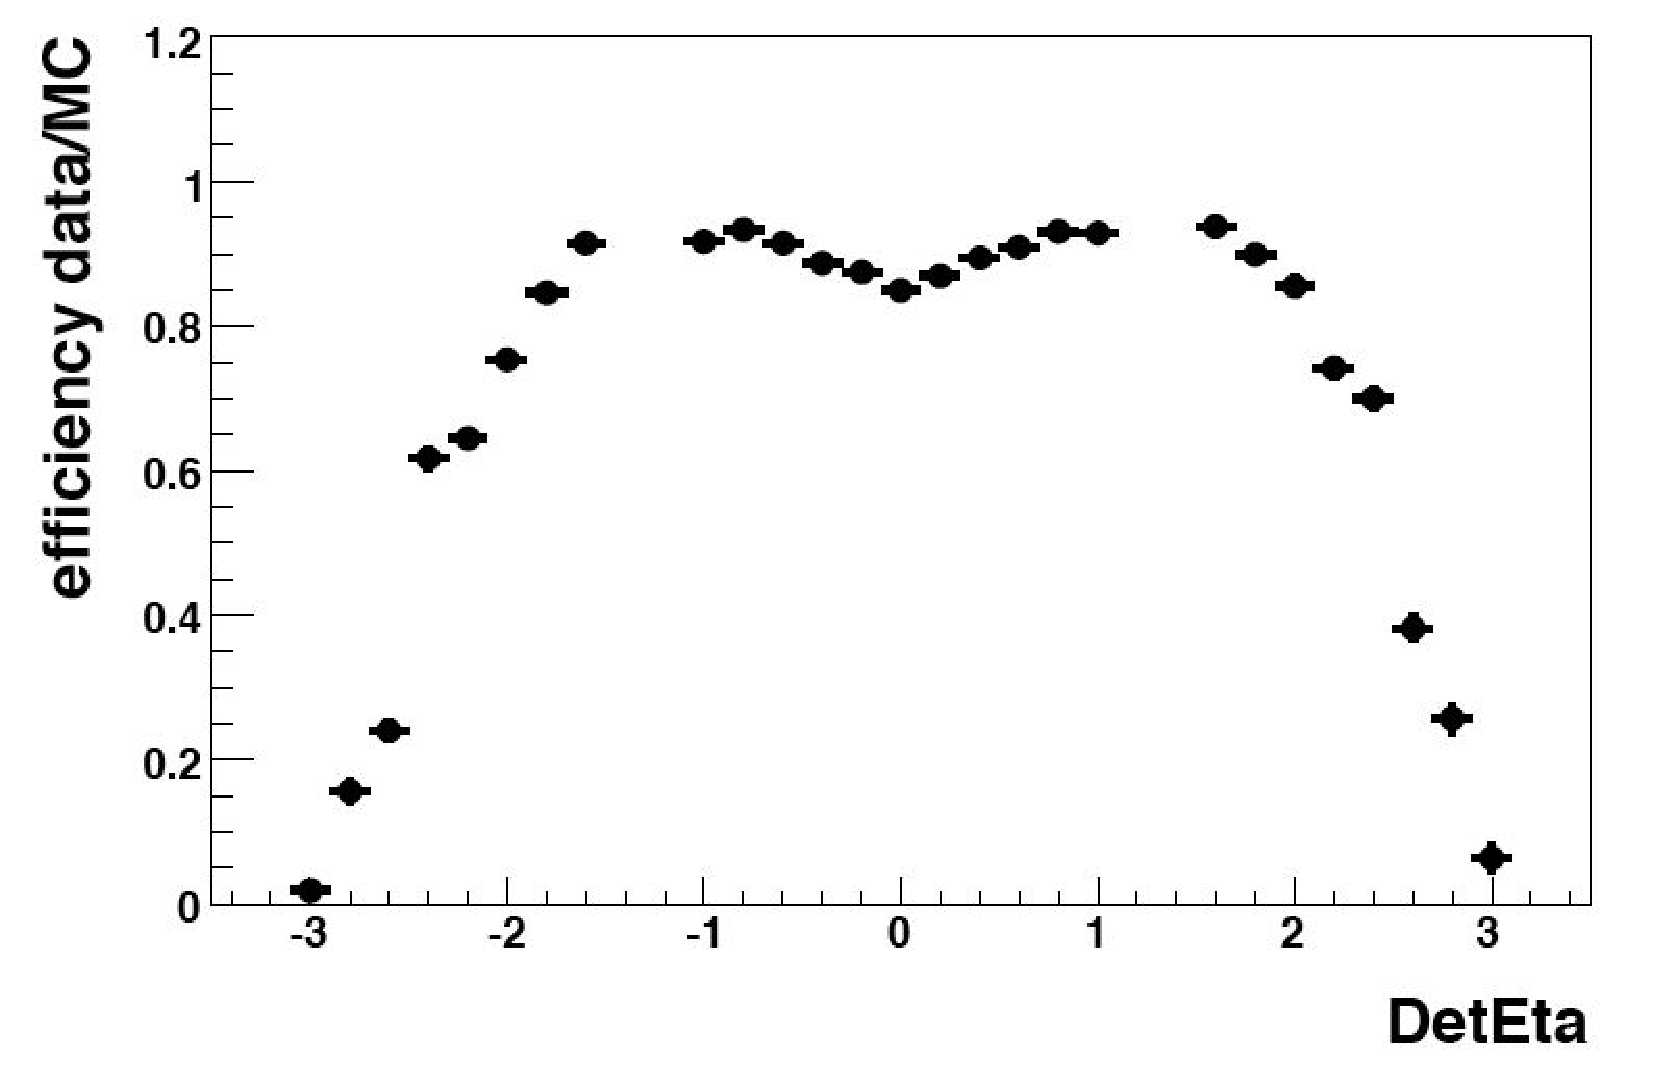
\includegraphics[width=0.49\textwidth]{eps/Reco/Electron_Likelihood_scale.eps}
\end{center}
\vspace{-0.1in}
\caption{Electron reconstruction efficiency as measured in $Z\rightarrow ee$ data (red) and Monte Carlo (blue) events (left) and Monte Carlo correction factor as a function of electron $p_{T}$ (right)~\cite{electron}.}
\label{electronlikelihoodeffscale}
\end{figure}

\subsection{Primary Interaction Vertex}

The primary interaction vertex efficiency is measured using $Z\rightarrow \mu\mu$ data and Monte Carlo events and the correction factor is defined as the ratio of the two efficiencies. The primary vertex reconstruction efficiency in data is shown in Fig.~\ref{pveff}. No correction to the Monte Carlo primary vertices is applied.

\begin{figure}[!h!tbp]
\begin{center}
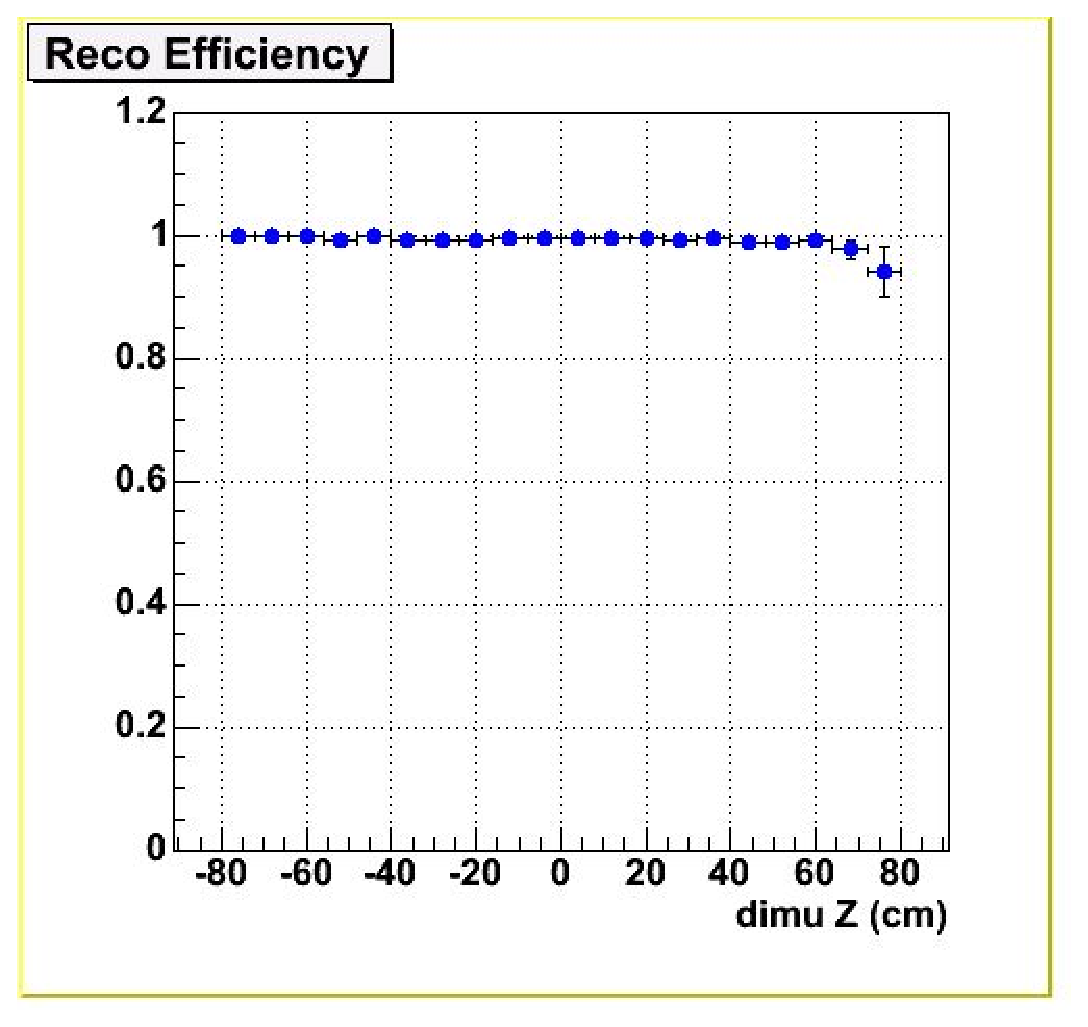
\includegraphics[width=0.65\textwidth]{eps/Reco/PV_Reco.eps}
\end{center}
\vspace{-0.1in}
\caption{Primary vertex reconstruction as measured on $Z \rightarrow ee$ data events. The efficiencies are shown as a function of the longitudinal primary vertex position~\cite{pv}.}
\label{pveff}
\end{figure}

\subsection{Jets}

Jets produced in the Monte Carlo simulation exhibit an overestimation of energy resolution, energy scale, and reconstruction efficiency. A procedure called SSR (Smearing, Shifting, and Removing) was designed to properly account for each of these relative differences between data and Monte Carlo~\cite{ssr}.

Jet energy resolution, energy scale, and reconstruction efficiency in the data and Monte Carlo are studied in back-to-back photon+jet events. In these events a variable called the transverse momentum imbalance, as shown in Eq.~\ref{deltaS}, is used to study these effects.

\begin{equation}
\label{deltaS}
\Delta S = \frac{p_{T}^{\rm{Jet}} - p_{T}^{\rm{\gamma}}}{p_{T}^{\rm{Jet}}}
\end{equation}

To determine the difference in the jet energy reconstruction efficiency in data and Monte Carlo, the $\Delta S$~distribution is determined in several regions of photon $p_{T}$ and fit to a Gaussian convoluted with a jet reconstruction efficiency function as shown in Eq.~\ref{deltaSfit}.

\begin{equation}
\label{deltaSfit}
f(\Delta S) = N \times \left( 1 + erf  \left[ \frac{\Delta S - \alpha}{\sqrt{2} \beta} \right] \right) \times \mathrm{exp} \left\{ -\frac{(\Delta S - \Delta S_{0})^{2}}{2\sigma^{2}} \right\}
\end{equation}

\noindent Where the constants $\{ \alpha, \beta \}$~characterize the jet reconstruction efficiency, $\Delta S_{0}$ yields information about the relative jet energy scale, and $\sigma$~characterizes the relative jet energy resolution.

To correct for the difference in jet energy resolution between data and Monte Carlo the Monte Carlo jet $p_{T}$ is smeared by a Gaussian with a width shown in Eq.~\ref{jetsmear}. If the generated jet $p_{T}$ is less than 15 GeV the jet is removed from the event. 
\begin{equation}
\label{jetsmear}
\sigma_{\rm{smear}} = \sqrt{ \sigma_{\rm{Data}}^{2}  - \sigma_{\rm{MC}}^{2}}
\end{equation}

The relative difference between the jet energy scale in data and Monte Carlo was found to be negligible ($\Delta S^{\rm{data}}_{0} \approx \Delta S^{\rm{MC}}_{0}$). The improved $\Delta S$ agreement between data and Monte Carlo after smearing and jet removal for two photon $p_{T}$ ranges can be seen in Fig.~\ref{jssr}.

\begin{figure}[!h!tbp]
\begin{center}
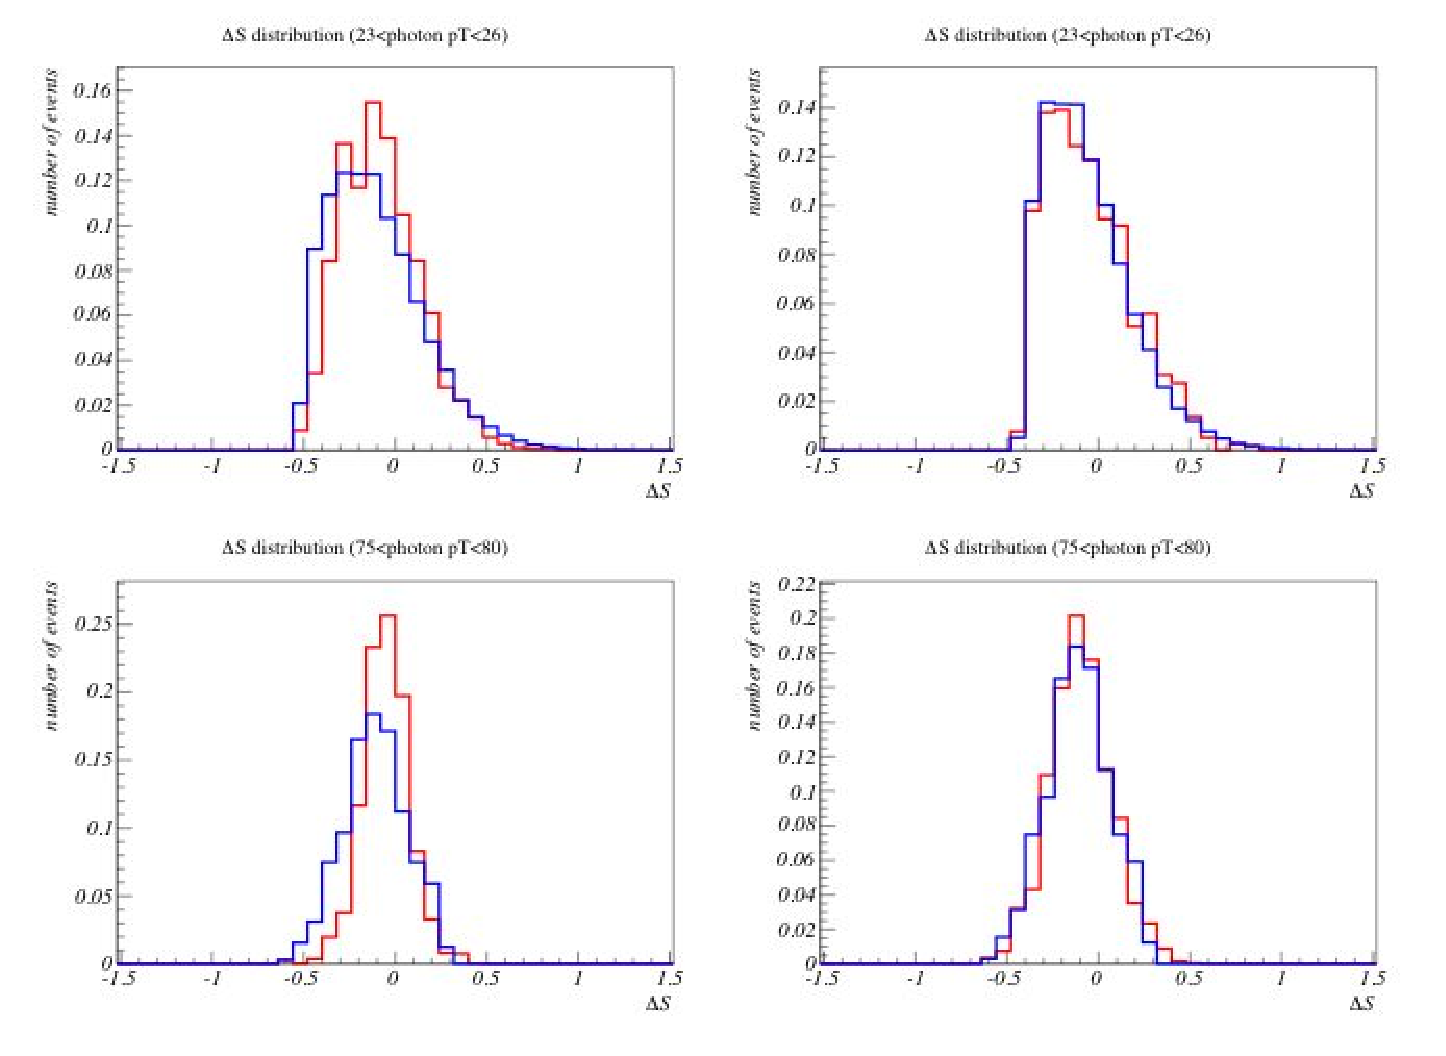
\includegraphics[width=1.0\textwidth]{eps/Reco/SSR.eps}
\end{center}
\vspace{-0.1in}
\caption{$p_{T}$ imbalance ($\Delta S$) distribution before (left) and after (right) jet smearing and removal are applied for two photon $p_{T}$ regions: $23<p_{T}^{\gamma}<26$ (top) and $75<p_{T}^{\gamma}<80$ (bottom). The data is shown in blue and the Monte Carlo is shown in red~\cite{ssr}.}
\label{jssr}
\end{figure}


\subsection{$B$-jets}

Due to large differences between data and Monte Carlo in tracking related quantities the $B$-tagging algorithms can not be directly applied to Monte Carlo events. Instead a probability for the algorithm to tag a $B$-jet, charm-jet, or a light jet is measured and applied to the Monte Carlo events~\cite{bid}. These probabilities, called tag-rate functions (TRF), are measured in data and Monte Carlo events and scaled to reproduce the expected $B$-jet, charm-jet and light-jet tagging efficiencies in data. As explained in Section~\ref{bidreco} all jets must have at least two associated tracks with $p_{T}>1$~GeV before $B$-tagging can be applied. This requirement is known as jet taggability ($\varepsilon_{\rm{Taggability}}$) and the product this quantity with the TRF yields the probability that a jet is $B$-tagged.

\begin{equation}
P_{\rm{tag}}(\vec{x}) = \varepsilon^{\rm{Taggability}}(\vec{x}) \times TRF(\vec{x})
\end{equation}

Using this per-jet tagging probability the probability that one jet is tagged in an event with $N$ jets is shown in Eq.~\ref{onetag} and probability that two jets are tagged is shown in Eq.~\ref{twotag}. These probabilities are applied to the Monte Carlo while the tagging algorithm is applied directly to the data.

\begin{equation}
\label{onetag}
P_{\rm{1-tag}} = \sum_{i=1}^{N_{\rm{jets}}} P_{\rm{tag},i} \prod_{i \neq j}^{N_{\rm{jets}}} ( 1 - P_{\rm{tag},j} )
\end{equation}

\begin{equation}
\label{twotag}
P_{\rm{2-tags}} = \sum_{i=1}^{N_{\rm{jets}}} P_{\rm{tag},i} \sum_{i \neq j}^{N_{\rm{jets}}} P_{\rm{tag},j} \prod_{k \neq i \neq j}^{N_{\rm{jets}}} ( 1 - P_{\rm{tag},k} )
\end{equation}

The $B$-jet and light-jet neural network tagging efficiencies in data are measured using a $B$-tagging algorithm that is relatively uncorrelated with the NN tagger on two different data samples. The first data sample is a relatively loose $B$-jet enriched sample requiring at least one muon with $p_{T}>4$~GeV inside a $\Delta R=0.7$ cone size jet. The presence of the muon within the jet represents a possible semi-leptonic $B$ decay. The second data sample is highly enriched in $B$-jets requiring at least two jets where one of the jets is required to have a jet impact parameter probability less than 0.5. The jet impact parameter probability is a measure of the likelihood that the jet originates from the primary interaction vertex. Large values of this quantity imply the jet originated from the hard scatter and low values indicate the jet originated from a displaced vertex. The second $B$-jet tagging algorithm used is the soft lepton tagger (SLT), which requires a muon to be reconstructed inside a jet. This algorithm is relatively uncorrelated with the NN tagger because it tags based on semi-leptonic $B$ meson decays ( e.g. $B\rightarrow D\ell\nu$ ), while the NN tagger uses information based on the displaced vertex from the $B$ decay. Using the correlation between the taggers, as measured in Monte Carlo, and the correlation between the data samples, a system of eight equations with eight unknowns can constructed. This system is then solved yielding the $B$-jet and light-jet tagging efficiencies with uncertainties in data events enriched in semi-leptonic $B$ decays.

% The $B$-jet tagging efficiency has a quite complex structure resulting from geometry of the detector and tracking inefficiencies. To avoid statistical fluctuations in the efficiency measurement, the total $B$-jet tagging efficiency is parameterized in jet $p_{T}$ and $\eta$ using the functional form shown in Eq.~\ref{btageff}.

%\begin{equation}
%\label{btageff}
%\varepsilon^{\rm{Data}}_{b\rightarrow\mu}(p_{T}, \eta) = \frac{1}{\varepsilon^{\rm{All}}} \times \left[ %\frac{c}{1+ae^{-bp_{T}}} \right] \times \left[ d + e\eta + f\eta^{2} + g\eta^{3} + h\eta^{4} \right]
%\end{equation}

The $B$-jet tagging efficiency for Monte Carlo events with a semi-leptonic $B$ decay is also measured and the ratio of the data to the Monte Carlo efficiency is used as the correction factor to the Monte Carlo. The $B$-jet tag-rate function for a Monte Carlo event with an inclusive $B$ meson decay is defined as the product of the inclusive $B$-jet tagging efficiency in Monte Carlo with the correction factor as shown in Eq.~\ref{btageff_mc}.

\begin{equation}
\label{btageff_mc}
\rm{TRF}_{b}(p_{T}, \eta) = \varepsilon_{b\rightarrow\rm{INC}}^{\rm{MC}} \times \frac{\varepsilon^{\rm{Data}}_{b\rightarrow\mu}}{\varepsilon^{\rm{MC}}_{b\rightarrow\mu}}
\end{equation}

The charm-jet tagging efficiency is measured using a similar approach with an additional input from the Monte Carlo for the relative inclusive charm-jet to $B$-jet tagging efficiency. The combined charm-jet TRF is shown in Eq.~\ref{ctageff_mc}

\begin{equation}
\label{ctageff_mc}
\rm{TRF}_{c}(p_{T}, \eta) = \varepsilon_{b\rightarrow\rm{INC}}^{\rm{MC}} \times \frac{\varepsilon^{\rm{Data}}_{b\rightarrow\mu}}{\varepsilon^{\rm{MC}}_{b\rightarrow\mu}} \times \frac{\varepsilon^{\rm{MC}}_{c\rightarrow\rm{INC}}}{\varepsilon^{\rm{MC}}_{b\rightarrow\rm{INC}}}
\end{equation}

The tag-rate functions for $B$-jets and charm-jets as a function of $p_{T}$ are shown in Fig.~\ref{bctrf}.

\begin{figure}[!h!tbp]
\begin{center}
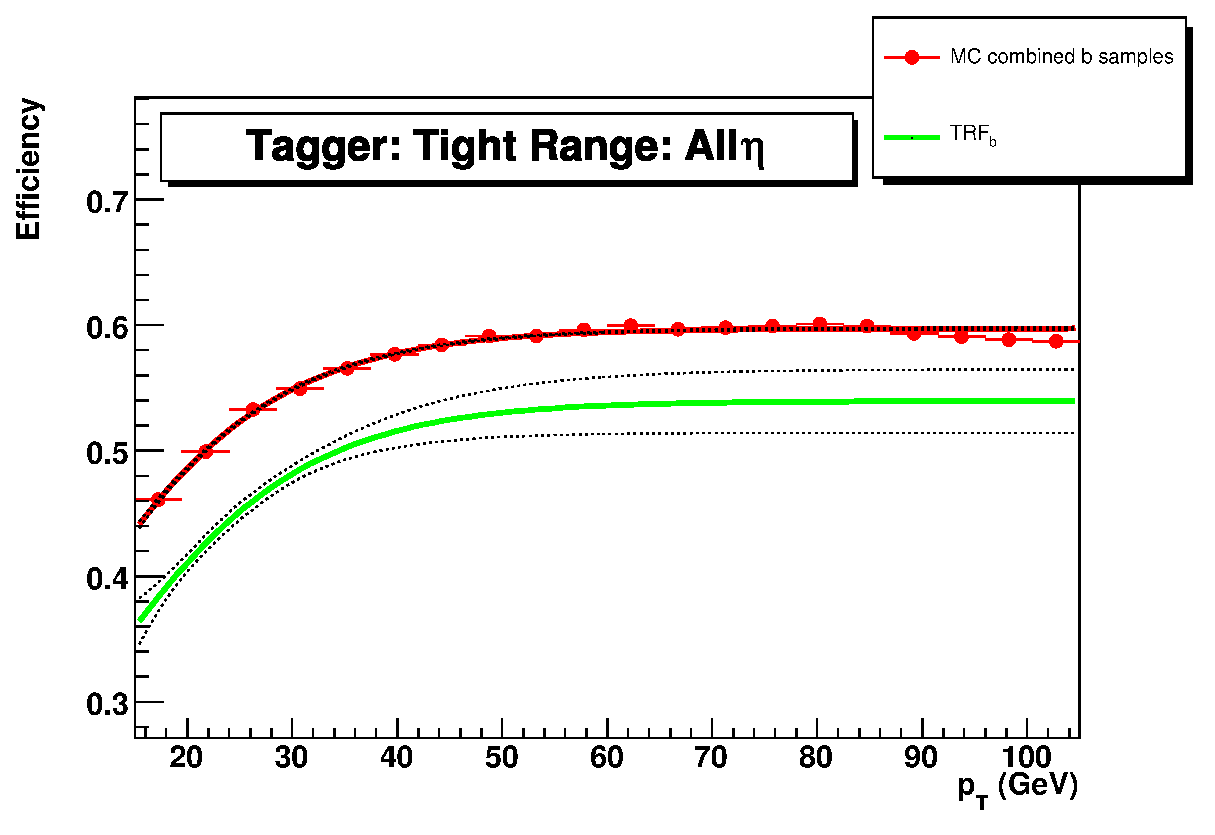
\includegraphics[width=0.48\textwidth]{eps/Systematics/trf_b_0.775_pt.eps}
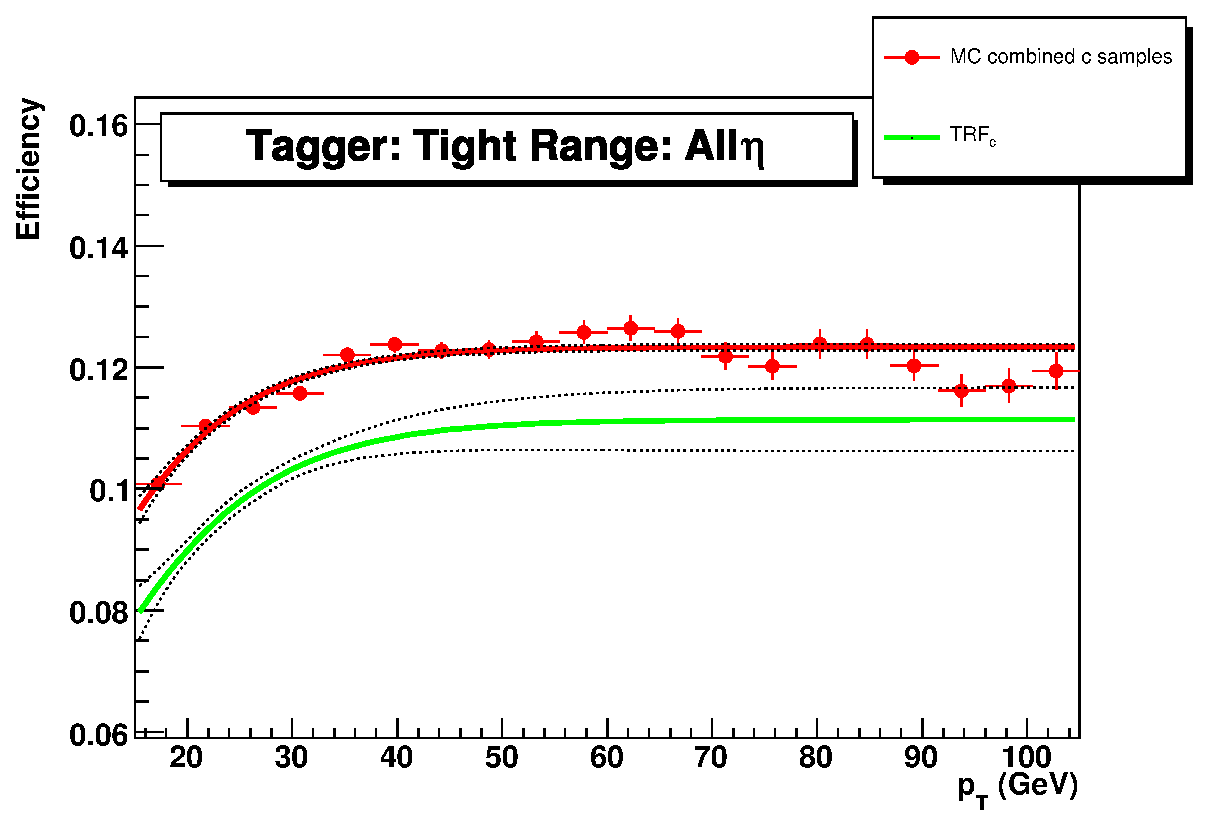
\includegraphics[width=0.48\textwidth]{eps/Systematics/trf_c_0.775_pt.eps}
\end{center}
\vspace{-0.1in}
\caption{Neural network $B$-jet tagger efficiency (green line) and $1\sigma$~error bands (dashed lines) jet $p_{T}$ and $B$-jets (left) and charm-jets (right)~\cite{bid}.}
\label{bctrf}
\end{figure}



The light-jet tagging efficiency, sometimes called the fake tag-rate (FTR), is calculated from the product of the negative tag-rate (NTR) and two Monte Carlo correction factions. The negative tag-rate is the efficiency for which a jet resulting from light flavor partons is mistaken for a $B$-jet. This typically occurs due to poor track or primary interaction vertex resolution in the event. A negative tag (NT) is found when the scalar product of the vector defined by the jet axis and the vector defined by the sum of the track vectors is negative. A positive tag is the case when the scalar product is greater than zero. Fig.~\ref{negativetag} shows the scalar products divided by the their error for $B$-jets and light jets in the Monte Carlo. 

\begin{figure}[!h!tbp]
\begin{center}
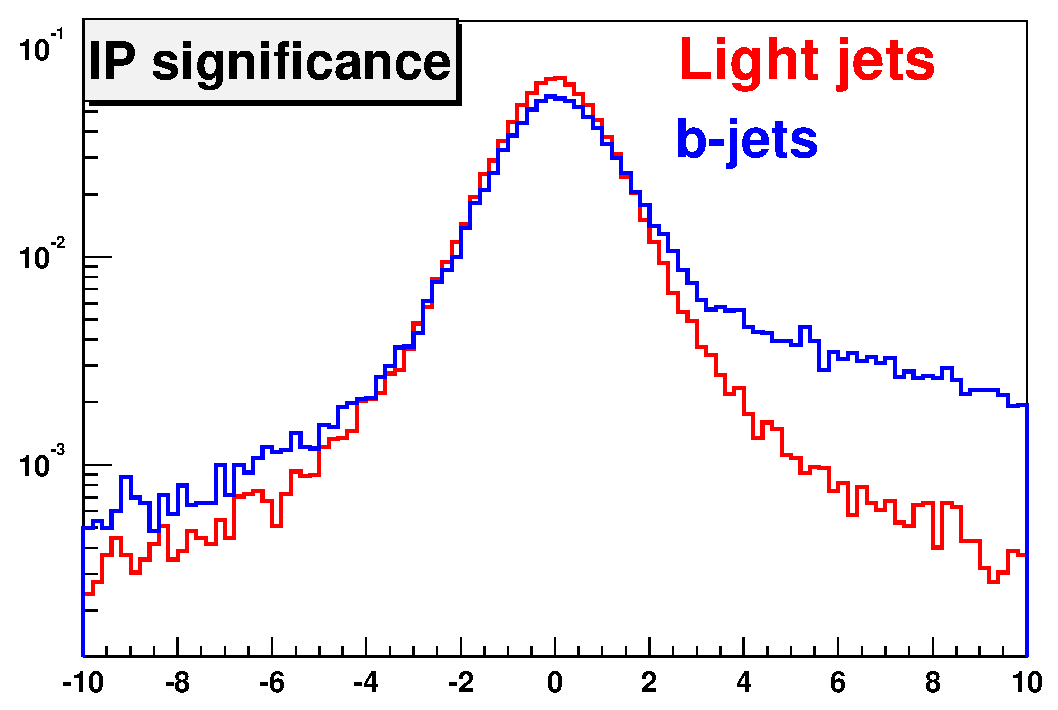
\includegraphics[width=0.65\textwidth]{eps/Reco/NegativeTag.eps}
\end{center}
\vspace{-0.1in}
\caption{The impact parameter significance for $B$-jets and light jets. The IP significance is defined as the signed scalar product of the jet-axis and vector defined by the tracks of the displaced vertex divided by the error on that measurement~\cite{aran}.}
\label{negativetag}
\end{figure}

The negative tag-rate is measured in data events with little bias towards heavy-flavor events. The NTR has two corrections which must be applied to remove any effects from heavy-flavor events that also receive a negative tag and a correction factor for the ratio of negative to positive tags for light-jets. The first correction factor is measured on $g\rightarrow b\bar{b}$ and $g\rightarrow c\bar{c}$ Monte Carlo and is defined as the ratio of the number of light-jets with a negative tag to the total number of negative tags. The second correction factor is measured on $g\rightarrow (udsg)(udsg)$ Monte Carlo and is defined as the ratio of the number of light-jets with a positive tag to the number of light-jets with a negative tag. The combined light-jet fake tag-rate function is shown in Eq.~\ref{lightjet_eff}

\begin{equation}
\label{lightjet_eff}
\rm{FTR}(p_{T}, \eta) = \rm{NTR}^{\rm{Data}} \times \frac{N^{\rm{MC}}_{l\rightarrow \rm{NT}}}{N^{\rm{MC}}_{l\rightarrow\rm{NT}} + N^{\rm{MC}}_{c\rightarrow\rm{NT}} + N^{\rm{MC}}_{b\rightarrow\rm{NT}} } \times \frac{N^{\rm{MC}}_{l\rightarrow\rm{PT}}}{N^{\rm{MC}}_{l\rightarrow\rm{NT}}}
\end{equation}